\subsection{PRODUCT DECOMPOSITION OF THE AFFINE SPACE E}

We retain the notation of Prop. 5. For \(0 \leqslant p \leqslant s\) , let \(\mathbf{E}_p\) be the set of orbits of the group \(\mathbf{T}_p'\) in \(\mathbf{E}\) , and let \(\varphi_p\) be the canonical map from \(\mathbf{E}\) to \(\mathbf{E}_p\) . The action of \(\mathbf{T}\) on \(\mathbf{E}\) passes to the quotient; in particular, \(\mathbf{T}_p\) acts on \(\mathbf{E}_p\) and it is immediate (for example by taking an origin in \(\mathbf{E}\) ) that \(\mathbf{E}_p\) is an affine space admitting \(\mathbf{T}_p\) as its space of translations. Put \(\mathbf{E}' = \mathbf{E}_0 \times \cdots \times \mathbf{E}_s\) ; this is an affine space having \(\mathbf{T} = \mathbf{T}_0 \oplus \cdots \oplus \mathbf{T}_s\) as its space of translations. Let \(\varphi : \mathbf{E} \to \mathbf{E}'\) be the product map of the \(\varphi_p\) ; since \(\varphi\) commutes with the action of \(\mathbf{T}\) , this is a bijection and even an isomorphism of affine spaces. In what follows, we identify \(\mathbf{E}\) and \(\mathbf{E}'\) by means of \(\varphi\) ; the map \(\varphi_p\) is then identified with the canonical projection of \(\mathbf{E}'\) onto \(\mathbf{E}_p\) .

Since W leaves \(T_{p}^{\prime}\) stable, the action of W on E passes to the quotient and defines an action of W on \(E_{p}\) (for \(0 \leqslant p \leqslant s\) ), and hence by restriction an action of \(W_{p}\) on \(E_{p}\) (for \(1 \leqslant p \leqslant s\) ). On the other hand, let C be a chamber, let \(i \in I\) and let p be the integer such that \(i \in J_{p}\) . For any \(x \in E\) , we have

\[
s _ {i} (\mathrm{C}) (x) = x - \lambda . e _ {i} (\mathrm{C}) \quad \text { with } \quad \lambda \in \mathbf {R}.
\]

Since \(e_i \in \mathbf{T}_q'\) for \(q \neq p\) , it follows that

\[
\varphi_ {q} (w (x)) = \varphi_ {q} (x) \text {for} x \in \mathrm{E}, w \in \mathrm{W} _ {p}; 0 \leqslant q \leqslant s \text {and} q \neq p.
\]

Consequently, if \(w = w_{1} \ldots w_{s} \in \mathrm{W}\) with \(w_{p} \in \mathrm{W}_{p}\) for \(1 \leqslant p \leqslant s\) , then

\[
w \left(\left(x _ {0}, \dots , x _ {s}\right)\right) = \left(x _ {0}, w _ {1} \left(x _ {1}\right), \dots , w _ {s} \left(x _ {s}\right)\right)\tag{5}
\]

for all \(x_{p} \in E_{p}\) for \(0 \leqslant p \leqslant s\) . In other words, the action of W on \(E = E'\) is exactly the product of the actions of the \(W_{p}\) on \(E_{p}\) (we put \(W_{0} = \{1\}\) ). It follows that \(W_{p}\) acts faithfully on \(E_{p}\) and that \(W_{p}\) can be identified with a group of displacements of the euclidean space \(E_{p}\) (the space \(T_{p}\) of translations of \(E_{p}\) being provided, of course, with the scalar product induced by that on T).

PROPOSITION 6. (i) The group \(W_{p}\) is a group of displacements of the euclidean affine space \(E_{p}\) ; it is generated by reflections; provided with the discrete topology, it acts properly on \(E_{p}\) ; it is irreducible.

\begin{enumerate}
\def\labelenumi{(\roman{enumi})}
\setcounter{enumi}{1}
\tightlist
\item
  Let \(\mathfrak{H}_p\) be the set of hyperplanes \(\mathrm{H}\) of \(\mathrm{E}_p\) such that \(s_{\mathrm{H}} \in \mathrm{W}_p\) . The set \(\mathfrak{H}\) consists of the hyperplanes of the form
\end{enumerate}

\[
\mathrm{H} = \mathrm{E} _ {0} \times \mathrm{E} _ {1} \times \dots \times \mathrm{E} _ {p - 1} \times \mathrm{H} _ {p} \times \mathrm{E} _ {p + 1} \times \dots \times \mathrm{E} _ {s},
\]

with \(p = 1,\dots ,s\) and \(\mathrm{H}_p\in \mathfrak{H}_p\)

\begin{enumerate}
\def\labelenumi{(\roman{enumi})}
\setcounter{enumi}{2}
\tightlist
\item
  Every chamber C is of the form \(E_{0} \times C_{1} \times \cdots \times C_{s}\) , where for each p the set \(C_{p}\) is a chamber defined in \(E_{p}\) by the set of hyperplanes \(H_{p}\) ; moreover, the walls of \(C_{p}\) are the hyperplanes \(\varphi_{p}(H_{i}(C))\) for \(i \in J_{p}\) .
\end{enumerate}

Let \(\mathbf{C}\) be a chamber. Put \(\mathrm{H}_i = \mathrm{H}_i(\mathrm{C})\) , \(e_i = e_i(\mathrm{C})\) and \(s_i = s_i(\mathrm{C})\) for \(i \in \mathbb{I}\) (in the notation of no. 4).

\begin{enumerate}
\def\labelenumi{(\roman{enumi})}
\tightlist
\item
  Let \(i\) be in \(\mathbf{J}_p\) ; since \(e_i \in \mathrm{T}_p\) and \(\mathrm{T}\) is the direct sum of the mutually orthogonal subspaces \(\mathrm{T}_0, \mathrm{T}_1, \ldots, \mathrm{T}_s\) , the hyperplane of \(\mathrm{T}\) orthogonal to \(e_i\) is of the form \(\mathrm{L}_i + \mathrm{T}_p'\) , where \(\mathrm{L}_i\) is the hyperplane of \(\mathrm{T}_p\) orthogonal to \(e_i\) . The affine hyperplane \(\mathrm{H}_i\) of \(\mathrm{E}\) is of the form \(\mathrm{L}_i + \mathrm{T}_p' + x\) , with \(x \in \mathrm{E}\) , and we have
\end{enumerate}

\[
\mathrm{H} _ {i} = \mathrm{E} _ {0} \times \mathrm{E} _ {1} \times \dots \times \mathrm{E} _ {p - 1} \times \mathrm{H} _ {i} ^ {\prime} \times \mathrm{E} _ {p + 1} \times \dots \times \mathrm{E} _ {s}\tag{6}
\]

with \(H_{i}^{\prime}=L_{i}+\varphi_{p}(x)=\varphi_{p}(H_{i})\) . It is now immediate that \(s_{i}\) acts in \(E_{p}\) by the reflection associated to the hyperplane \(H_{i}^{\prime}\) of \(E_{p}\) . Thus, the group \(W_{p}\) is a group of displacements generated by reflections in \(E_{p}\) ; the verification of the properness criterion (D'2) is immediate. Finally, Prop. 5, (v) shows that \(W_{p}\) is irreducible. This proves (i).

\begin{enumerate}
\def\labelenumi{(\roman{enumi})}
\setcounter{enumi}{1}
\tightlist
\item
  By the Cor. of Th. 1, the set \(\mathfrak{H}_p\) consists of the hyperplanes of the form \(w_p(\mathrm{H}_i')\) for \(i\) in \(\mathrm{J}_p\) and \(w_p\) in \(\mathrm{W}_p\) . Further, if \(w = w_1 \ldots w_s\) with \(w_p \in \mathrm{W}_p\) for all \(p\) , formulas (5) and (6) imply that
\end{enumerate}

\[
w (\mathrm{H} _ {i}) = \mathrm{E} _ {0} \times \mathrm{E} _ {1} \times \dots \times \mathrm{E} _ {p - 1} \times w _ {p} (\mathrm{H} _ {i} ^ {\prime}) \times \mathrm{E} _ {p + 1} \times \dots \times \mathrm{E} _ {s},\tag{7}
\]

from which (ii) follows immediately.

\begin{enumerate}
\def\labelenumi{(\roman{enumi})}
\setcounter{enumi}{2}
\tightlist
\item
  Let \(i\) be in \(\mathbf{J}_p\) ; by formula (6), the open half-space \(D_i\) bounded by \(\mathbf{H}_i\) and containing \(C\) is of the form
\end{enumerate}

\[
\mathrm{D} _ {i} = \mathrm{E} _ {0} \times \mathrm{E} _ {1} \times \dots \times \mathrm{E} _ {p - 1} \times \mathrm{D} _ {i} ^ {\prime} \times \mathrm{E} _ {p + 1} \times \dots \times \mathrm{E} _ {s},
\]

where \(D_{i}^{\prime}\) is an open half-space bounded by \(H_{i}^{\prime}\) in \(E_{p}\) . Put \(C_{p} = \bigcap_{i \in J_{p}} D_{i}^{\prime}\) ; since \(C = \bigcap_{i \in I} D_{i}\) , it follows immediately that

\[
\mathrm{C} = \mathrm{E} _ {0} \times \mathrm{C} _ {1} \times \dots \times \mathrm{C} _ {s};
\]

consequently, none of the sets \(C_{p}\) is empty, and since C does not meet any hyperplane belonging to H, the set \(C_{p}\) does not meet any hyperplane belonging to \(H_{p}\) . Prop. 5 of §1, no. 3 now shows that \(C_{p}\) is one of the chambers defined by \(H_{p}\) in \(E_{p}\) . By using Prop. 4 of §1, no. 2, it is easy to see that the walls of \(C_{p}\) are the hyperplanes \(H_{i}^{\prime} = \varphi_{p}(H_{i})\) for \(i \in J_{p}\) .

\subsection{STRUCTURE OF CHAMBERS}

Let \(\mathbf{C}\) be a chamber, let \(\mathfrak{M}\) be the set of walls of \(\mathbf{C}\) , and for \(\mathrm{H} \in \mathfrak{M}\) let \(e_{\mathrm{H}}\) be the unit vector orthogonal to \(\mathrm{H}\) on the same side of \(\mathrm{H}\) as \(\mathbf{C}\) .

PROPOSITION 7. Assume that the group W is essential and finite. Then:

\begin{enumerate}
\def\labelenumi{(\roman{enumi})}
\item
  There exists a unique point \(a\) of \(\mathbf{E}\) invariant under \(\mathbf{W}\) .
\item
  The family \((e_{\mathsf{H}})_{\mathsf{H}\in \mathfrak{M}}\) is a basis of \(\mathrm{T}\) .
\item
  The chamber C is the open simplicial cone with vertex a defined by the basis \((e_{\mathrm{H}}^{\prime})_{\mathrm{H}\in \mathfrak{M}}\) of T such that \((e_{\mathrm{H}}|e_{\mathrm{H}'}') = \delta_{\mathrm{HH}'}\) .
\item
  By Prop. 4 of no. 6, there exists a point \(a \in E\) invariant under W. Let \(t \in T\) be such that \(t + a\) is invariant under W. For all \(w \in W\) ,
\end{enumerate}

\[
\mathrm{U} (w). t + a = w (t + a) = t + a,
\]

so \(\mathrm{U}(w).t = t\) ; since \(\mathrm{W}\) is essential, this implies that \(t = 0\) , showing the uniqueness of \(a\) .

\begin{enumerate}
\def\labelenumi{(\roman{enumi})}
\setcounter{enumi}{1}
\item
  Since W is essential, \(T = T_{1}\) in the notation of no. 7, and Prop. 5, (iv) shows that the family \((e_{\mathrm{H}})_{\mathrm{H}\in\mathfrak{M}}\) generates the vector space T. The existence of a point of E invariant under W shows that the family \((e_{\mathrm{H}})_{\mathrm{H}\in\mathfrak{M}}\) is free (no. 6, Prop. 4).
\item
  Let \(a\) be the unique point of \(\mathbf{E}\) invariant under \(\mathbf{W}\) . Since \((e_{\mathrm{H}})_{\mathrm{H}\in \mathfrak{M}}\) is a basis of \(\mathbf{T}\) , and since the scalar product is a non-degenerate bilinear form on \(\mathbf{T}\) , there exists a unique basis \((e_{\mathrm{H}}^{\prime})_{\mathrm{H}\in \mathfrak{M}}\) of \(\mathbf{T}\) such that \((e_{\mathrm{H}}|e_{\mathrm{H}'}') = \delta_{HH'}\) for \(\mathrm{H},\mathrm{H}'\) in \(\mathfrak{M}\) . Every point \(x\) of \(\mathbf{E}\) can be written uniquely in the form \(x = t + a\) with \(t = \sum_{\mathrm{H}\in \mathfrak{M}}\xi_{\mathrm{H}}.e_{\mathrm{H}}'\) and the \(\xi_{\mathrm{H}}\) real. Then \(x\) belongs to \(\mathbf{C}\) if and only if, for every hyperplane \(\mathrm{H}\in \mathfrak{M}\) , \(x\) is on the same side of \(\mathbf{H}\) as \(e_{\mathrm{H}}\) , or in other words \((t|e_{\mathrm{H}}) = \xi_{\mathrm{H}}\) is strictly positive. Hence (iii).
\end{enumerate}

PROPOSITION 8. Assume that the group W is essential, irreducible and infinite. Then:

\begin{enumerate}
\def\labelenumi{(\roman{enumi})}
\item
  No point of E is invariant under W.
\item
  We have \(\operatorname{Card} \mathfrak{M} = \dim T + 1\) , and there exist real numbers \(c_{\mathrm{H}} > 0\) such that \(\sum_{\mathrm{H} \in \mathfrak{M}} c_{\mathrm{H}} \cdot e_{\mathrm{H}} = 0\) . If the real numbers \(c_{\mathrm{H}}'\) are such that \(\sum_{\mathrm{H} \in \mathfrak{M}} c_{\mathrm{H}}' \cdot e_{\mathrm{H}} = 0\) , there exists a real number \(\xi\) such that \(c_{\mathrm{H}}' = \xi c_{\mathrm{H}}\) for all H in \(\mathfrak{M}\) .
\item
  The chamber C is an open simplex.
\end{enumerate}

Assertion (i) follows from Prop. 4. On the other hand, since W is essential, the vectors \((e_{\mathrm{H}})_{\mathrm{H}\in\mathfrak{M}}\) generate T. We have \((e_{\mathrm{H}}|e_{\mathrm{H}^{\prime}})\leqslant0\) for \(H,H^{\prime}\in \mathfrak{M}\) and \(H\neq H^{\prime}\) (Prop. 3) and, since W is irreducible, there does not exist a partition of \(\mathfrak{M}\) into two disjoint subsets \(\mathfrak{M}^{\prime}\) and \(\mathfrak{M}^{\prime\prime}\) such that \(H^{\prime}\in \mathfrak{M}^{\prime}\) and \(H^{\prime\prime}\in \mathfrak{M}^{\prime\prime}\) imply that \((e_{\mathrm{H}^{\prime}}|e_{\mathrm{H}^{\prime\prime}})=0\) . We can thus apply Lemma 5 of no. 5, and case 1) of that lemma is excluded; indeed, the \(e_{H}\) are not linearly independent, since W has no fixed point. Assertion (ii) follows.

We now prove (iii). Number the walls of C as \(H_{0}, H_{1}, \ldots, H_{d}\) and put \(t_{m} = e_{H_{m}}\) . By (ii), the vectors \(t_{1}, \ldots, t_{d}\) form a basis of T, so the hyperplanes \(H_{1}, \ldots, H_{d}\) have a point \(a_{0}\) in common, and there exists a basis \((t_{1}^{\prime}, \ldots, t_{d}^{\prime})\) of T such that \((t_{m}|t_{n}^{\prime}) = \delta_{mn}\) ; moreover, again by (ii) there exist real numbers \(c_{1} > 0, \ldots, c_{d} > 0\) such that

\[
t _ {0} = - \left(c _ {1}. t _ {1} + \dots + c _ {d}. t _ {d}\right).
\]

Since the vector \(t_{0}\) is orthogonal to the hyperplane \(H_{0}\) , there exists a real number c such that \(H_{0}\) is the set of points \(x = t + a_{0}\) of E with \((t|t_{0}) = -c\) .

Every point of E can be written uniquely in the form \(x = t + a_{0}\) with \(t = \xi_{1}.t_{1}^{\prime} + \cdots + \xi_{d}.t_{d}^{\prime}\) and \(\xi_{1}, \ldots, \xi_{d}\) real. The point x belongs to C if and only if it is on the same side of \(H_{m}\) as \(t_{m}\) for \(0 \leqslant m \leqslant d\) ; this translates into the inequalities \((t|t_{1}) > 0, \ldots, (t|t_{d}) > 0\) , and \((t|t_{0}) > -c\) , or equivalently by \(\xi_{1} > 0, \ldots, \xi_{d} > 0\) , \(c_{1}\xi_{1} + \cdots + c_{d}\xi_{d} < c\) . Since C is non-empty, c \textgreater{} 0. Put \(a_{m} = a_{0} + \frac{c}{c_{m}}.t_{m}'\) for \(1 \leqslant m \leqslant d\) ; then the chamber C consists of the points of E of the form \(a_{0} + \sum_{m=1}^{d} \lambda_{m}.(a_{m} - a_{0})\) with \(\lambda_{1} > 0, \ldots, \lambda_{d} > 0\) and \(\lambda_{1} + \cdots + \lambda_{d} < 1\) , so C is the open simplex with vertices \(a_{0}, \ldots, a_{d}\) . Q.E.D.

Remarks. 1) Identify E with \(E_{0} \times E_{1} \times \cdots \times E_{s}\) and W with \(W_{1} \times \cdots \times W_{s}\) as in no. 8. By Prop. 6, the chamber C is then identified with

\[
\mathrm{E} _ {0} \times \mathrm{C} _ {1} \times \dots \times \mathrm{C} _ {s},
\]

where \(C_{p}\) is a chamber in \(E_{p}\) with respect to the set of hyperplanes \(H_{p}\) . By Props. 7 and 8, each of the chambers \(C_{1},\ldots,C_{s}\) is an open simplicial cone or an open simplex.

\begin{enumerate}
\def\labelenumi{\arabic{enumi})}
\setcounter{enumi}{1}
\tightlist
\item
  Assume that W is irreducible and essential. If H and \(H'\) are two walls of C, then \(m_{HH'} = +\infty\) if and only if \(e_{H} = -e_{H'}\) (Prop. 3). By Props. 7 and 8, this can happen only if H and \(H'\) are the only walls of C and E is of dimension 1. Thus, the only case in which one of the \(m_{HH'}\) is infinite is that in which E is of dimension 1 and the group W is generated by the reflections associated to two distinct points (cf.~§2, no. 4).
\end{enumerate}

In the general case, the entries of the Coxeter matrix associated to W are finite unless at least one of \(E_{1},\ldots,E_{s}\) is of the preceding type.

\subsection{SPECIAL POINTS}

Let L be the set of translations belonging to W and let \(\Lambda\) be the set of \(t \in T\) such that the translation \(x \mapsto t + x\) belongs to L. It is immediate that \(\Lambda\) is stable under U(W) and that L is a normal subgroup of W. Since W acts properly on E, the same holds for L, and it follows easily that \(\Lambda\) is a discrete subgroup of T. For any point x of E, denote by \(W_x\) the stabiliser of x in W.

PROPOSITION 9. Let \(a \in E\) . The following conditions are equivalent:

\begin{enumerate}
\def\labelenumi{(\roman{enumi})}
\item
  We have \(\mathrm{W} = \mathrm{W}_{a}.\mathrm{L}\) ;
\item
  The restriction of the homomorphism U to \(W_{a}\) is an isomorphism from \(W_{a}\) to \(\mathrm{U}(\mathrm{W})\) ;
\item
  For every hyperplane \(\mathbf{H} \in \mathfrak{H}\) , there exists a hyperplane \(\mathbf{H}' \in \mathfrak{H}\) parallel to \(\mathbf{H}\) and such that \(a \in \mathbf{H}'\) .
\end{enumerate}

It is clear that (i) \(\Leftrightarrow\) (ii), since L is the kernel of U and \(\mathrm{L} \cap \mathrm{W}_a = \{1\}\) .

Assume (i) and let \(\mathbf{H} \in \mathfrak{H}\) ; then \(s_{\mathbf{H}} \in \mathbf{W}_a\) . L so there exists a vector \(t \in \Lambda\) such that \(a = s_{\mathbf{H}}(a) + t\) ; the vector \(t\) is orthogonal to \(\mathbf{H}\) , and if \(\mathrm{H}' = \mathrm{H} + \frac{1}{2} t\) then \(s_{\mathbf{H}'}(x) = s_{\mathbf{H}}(x) + t\) for all \(x \in \mathbf{E}\) (cf.~§2, no. 4, Prop. 5). Since \(t \in \Lambda\) and \(s_{\mathbf{H}} \in \mathbf{W}\) , we have \(s_{\mathbf{H}'} \in \mathbf{W}\) , and so \(\mathrm{H}' \in \mathfrak{H}\) ; we also have \(a = s_{\mathbf{H}'}(a)\) , and so \(a \in \mathbf{H}'\) . Thus, (i) implies (iii).

Assume (iii). Let \(\mathrm{H} \in \mathfrak{H}\) ; take \(\mathrm{H}'\) as in (iii). Then \(s_{\mathrm{H}'}(a) = a\) , so \(s_{\mathrm{H}'} \in \mathrm{W}_a\) ; since \(\mathrm{H}\) is parallel to \(\mathrm{H}'\) , the element \(w = s_{\mathrm{H}'} s_{\mathrm{H}}\) of \(\mathrm{W}\) is a translation (§2, no. 4, Prop. 5), so \(w \in \mathrm{L}\) ; then \(s_{\mathrm{H}} = s_{\mathrm{H}'} w \in \mathrm{W}_a\) . L. Since \(\mathrm{W}\) is generated by the family \((s_{\mathrm{H}})_{\mathrm{H} \in \mathfrak{H}}\) , it follows that \(\mathrm{W} = \mathrm{W}_a\) . L and hence (iii) implies (i).

DEFINITION 1. A point \(a\) of \(E\) is special for \(W\) if it satisfies the equivalent conditions in Prop. 9.

It is clear that the set of special points of E is stable under W.

PROPOSITION 10. There exists a special point for W.

By Prop. 6 of no. 8, we need only consider the case when W is essential. The group U(W) of automorphisms of T is finite (cf.~no. 6, Th. 3) and \(U(s_{H})\) is an orthogonal reflection for every hyperplane H; moreover, U(W) is generated by the family \((U(s_{H}))_{H \in \mathfrak{H}}\). By Prop. 7 of no. 9, there exists a basis \((e_{i})_{i \in I}\) of T such that the group U(W) is generated by the set of reflections \((s_{i})_{i \in I}\) defined by

\[
s _ {i} (t) = t - 2 (t | e _ {i}). e _ {i}.
\]

The Cor. of Th. 1 of no. 2 shows that every reflection \(s \in \mathrm{U}(\mathrm{W})\) is of the form \(s = \mathrm{U}(s_{\mathrm{H}})\) with \(\mathrm{H} \in \mathfrak{H}\) . We can thus find in \(\mathfrak{H}\) a family of hyperplanes \((\mathbf{H}_i)_{i \in I}\) such that \(s_i = \mathrm{U}(s_{\mathrm{H}_i})\) for all \(i\) . Since the vectors \(e_i\) are linearly independent, there exists \(a \in E\) such that \(a \in H_i\) for all \(i \in I\) . We have \(s_{\mathrm{H}_i} \in W_a\) , so \(\mathrm{U}(\mathrm{W}) = \mathrm{U}(\mathrm{W}_a)\) , which means that \(W = W_a.L\) since \(L\) is the kernel of \(U\) . Thus, \(a\) is special.

When W is finite and essential, there is only one special point for W, namely the unique point invariant under W. Thus, the consideration of special points is interesting mainly when W is infinite.

PROPOSITION 11. Assume that W is essential. Let a be a special point for W. The chambers relative to \(W_{a}\) are the open simplicial cones with vertex a. For every chamber \(C'\) relative to \(W_{a}\) , there exists a unique chamber C relative to W contained in \(C'\) and such that \(a \in \overline{C}\) . The union of the \(w'(\overline{C})\) for \(w' \in W_{a}\) is a closed neighbourhood of a in E. Every wall of \(C'\) is a wall of C. If W is infinite and irreducible, the walls of C are the walls of \(C'\) together with an affine hyperplane not parallel to the walls of \(C'\) .

Let \(\mathfrak{H}'\) be the set of \(H \in \mathfrak{H}\) containing \(a\) . The group \(W_a\) is generated by the \(s_H\) for \(H \in \mathfrak{H}'\) (no. 3, Prop. 2). The chambers relative to \(W_a\) are the open simplicial cones with vertex \(a\) (no. 9, Prop. 7). Let \(C'\) be such a chamber and let \(U\) be a non-empty open ball with centre \(a\) not meeting any element of \(\mathfrak{H} - \mathfrak{H}'\) . Since \(a \in \overline{C'}\) , there exists a point \(b\) in \(U \cap C'\) . Then \(b \notin H\) for all \(H \in \mathfrak{H}\) , so \(b\) belongs to a chamber \(C\) relative to \(\mathfrak{H}\) . Since \(\mathfrak{H}' \subset \mathfrak{H}\) , we have \(C \subset C'\) . The set \(U \cap C'\) does not meet any \(H \in \mathfrak{H}\) and is convex, so \(U \cap C' \subset C\) ; thus \(a \in \overline{C}\) . Conversely, let \(C_1\) be a chamber relative to \(W\) contained in \(C'\) and such that \(a \in \overline{C}_{1}\) ; then \(C_{1}\) meets U and \(U \cap C_{1} \subset U \cap C' = U \cap C\) ; the chambers C and \(C_{1}\) , having a point in common, must coincide. For any \(w' \in W_{a}\) , we have \(w'(U) = U\) , so

\[
\mathrm{U} \cap w ^ {\prime} (\mathrm{C}) = w ^ {\prime} (\mathrm{U} \cap \mathrm{C}) = w ^ {\prime} (\mathrm{U} \cap \mathrm{C} ^ {\prime}) = \mathrm{U} \cap w ^ {\prime} (\mathrm{C} ^ {\prime});
\]

since the union of the \(w'(C)\) for \(w' \in W_a\) is dense in \(E\) , the union of the \(U \cap w'(C) = U \cap w'(C')\) is dense in \(U\) , and the union of the \(w'(\overline{C})\) for \(w' \in W_a\) thus contains \(U\) . Finally, if \(H\) is a wall of \(C'\) , there exist a point \(c \in U \cap H\) and an open neighbourhood \(V \subset U\) of \(c\) such that \(V \cap C'\) is the intersection of \(V\) and the open half-space bounded by \(H\) containing \(C'\) ; since \(V \cap C' = V \cap U \cap C' = V \cap U \cap C = V \cap C\) , it follows that \(H\) is a wall of \(C\) . If \(W\) is infinite and irreducible, \(C\) is an open simplex (no. 9, Prop. 8) and so has one more wall than the open simplicial cone \(C'\) .

COROLLARY. Assume that W is essential.

\begin{enumerate}
\def\labelenumi{(\roman{enumi})}
\item
  If \(a \in \mathbb{E}\) is special, there exists a chamber \(\mathbb{C}\) such that \(a\) is an extremal point of \(\overline{\mathbb{C}}\) .
\item
  If \(\mathrm{C}\) is a chamber, there exists an extremal point of \(\overline{\mathrm{C}}\) that is special.
\end{enumerate}

The first assertion follows from Prop. 11. The second follows from the first and the fact that W acts transitively on the set of chambers.

However, an extremal point of \(\overline{C}\) is not necessarily a special point for W (cf.~Chap. VI, Plate X, Systems \(B_{2}\) and \(G_{2}\) ).

Remark. 1) Assume that W is essential, irreducible and infinite and retain the notation of Prop. 11. Since U is an isomorphism from \(W_{a}\) to \(U(W)\) , it follows that the Coxeter graph of the group of displacements \(U(W)\) (which is generated by the reflections \(U(s_{H})\) for \(H \in \mathfrak{H}\) ) can be obtained from the Coxeter graph of W by omitting the vertex i corresponding to the unique wall of C that is not a wall of \(C'\) .

PROPOSITION 12. Assume that W is essential. Let a be a special point, let L(a) be the set of its transforms under the group of translations L, and let C be a chamber. Then \(\overline{C}\) meets L(a) in a unique point; this point is an extremal point of \(\overline{C}\) .

There exists a chamber \(C_{1}\) such that a is an extremal point of \(\overline{C}_{1}\) (Cor. of Prop. 11). Every chamber is of the form \(\mathbf{C}=tw^{\prime}(\mathbf{C}_{1})\) with \(w^{\prime}\in W_{a}\) and \(t\in L\) since \(W=W_{a}.L\) ; thus \(tw^{\prime}(a)=t(a)\in\mathrm{L}(a)\) is an extremal point of \(\overline{C}\) . On the other hand, \(\overline{C}\) cannot contain two distinct points of \(\mathrm{L}(a)\) since \(\overline{C}\) is a fundamental domain for W (no. 3, Th. 2).

Remark. 2) The set L(a) is contained in the set of special points, but in general is distinct from it (cf.~Chap. VI, §2, no. 2 and Plates I to VI).

\section{THE GEOMETRIC REPRESENTATION OF A COXETER GROUP}

In this paragraph, all the vector spaces considered are real vector spaces.

\subsection{FORM ASSOCIATED TO A COXETER GROUP}

Let \(S\) be a set and let \(M = (m(s, s')_{s, s' \in S})\) be a Coxeter matrix (Chap. IV, §1, no. 9) of type \(S\) . Recall that this means:

\begin{enumerate}
\def\labelenumi{(\arabic{enumi})}
\item
  The elements of \(M\) are integers or \(+\infty\) .
\item
  M is symmetric.
\item
  \(m(s, s) = 1\) for all s.
\item
  \(m(s, s') \geqslant 2\) for \(s \neq s'\) .
\end{enumerate}

Let \(\mathbf{E} = \mathbf{R}^{(\mathrm{S})}\) , let \((e_s)_{s \in S}\) be the canonical basis of \(\mathbf{E}\) , and let \(B_M\) be the bilinear form on \(\mathbf{E}\) such that

\[
\mathrm{B} _ {\mathrm{M}} (e _ {s}, e _ {s ^ {\prime}}) = - \cos \frac {\pi}{m (s , s ^ {\prime})}.
\]

The form \(B_{M}\) is symmetric. It is called the associated form of the matrix M. We have

\[
\mathrm{B} _ {\mathrm{M}} \left(e _ {s}, e _ {s}\right) = 1 \text {and} \mathrm{B} _ {\mathrm{M}} \left(e _ {s}, e _ {s ^ {\prime}}\right) \leqslant 0 \text {if} s \neq s ^ {\prime}.
\]

Let \(s \in S\) and let \(f_s\) be the linear form \(x \mapsto 2B_M(e_s, x)\) . We denote by \(\sigma_s\) the pseudo-reflection defined by the pair \((e_s, f_s)\) (cf.~§2, no. 1); since \(\langle e_s, f_s \rangle = 2\) , it is a reflection (§2, no. 2). We have

\[
\sigma_ {s} (x) = x - 2 \mathrm{B} _ {\mathrm{M}} (e _ {s}, x). e _ {s}
\]

and in particular

\[
\sigma_ {s} (e _ {s ^ {\prime}}) = e _ {s ^ {\prime}} + 2 \cos \frac {\pi}{m (s , s ^ {\prime})}. e _ {s}.
\]

Since \(e_{s}\) is not isotropic for \(B_{M}\) , the space E is the direct sum of the line \(Re_{s}\) and the hyperplane \(H_{s}\) orthogonal to \(e_{s}\) . Since \(\sigma_{s}\) is equal to -1 on \(Re_{s}\) and to 1 on \(H_{s}\) , it follows that \(\sigma_{s}\) preserves the form \(B_{M}\) . When S is finite and \(B_{M}\) is non-degenerate (a case to which we shall return in no. 8), it follows that \(\sigma_{s}\) is an orthogonal reflection ( \(\S2\) , no. 3).

\subsection{\texorpdfstring{THE PLANE \(E_{s,s'}\) AND THE GROUP GENERATED BY \(\sigma_{s}\) AND \(\sigma_{s'}\)}{THE PLANE E\_s,s' AND THE GROUP GENERATED BY sigma\_s AND sigma\_s'}}

In this number, we denote by \(s\) and \(s'\) two elements of \(S\) with \(s \neq s'\) . Put \(m = m(s, s')\) and denote by \(\mathrm{E}_{s,s'}\) the plane \(\mathbf{Re}_s \oplus \mathbf{Re}_{s'}\) .

PROPOSITION 1. The restriction of \(B_{M}\) to \(E_{s,s'}\) is positive, and it is nondegenerate if and only if \(m\) is finite.

Let \(z = xe_{s} + ye_{s'}\) , with \(x, y \in \mathbf{R}\) , be an element of \(E_{s,s'}\) . We have

\[
\begin{array}{r} B _ {M} (z, z) = x ^ {2} - 2 x y \cos \frac {\pi}{m} + y ^ {2} \\ = (x - y. \cos \frac {\pi}{m}) ^ {2} + y ^ {2} \sin^ {2} \frac {\pi}{m}, \end{array}
\]

which shows that \(\mathrm{B}_{\mathsf{M}}\) is positive on \(\mathrm{E}_{s,s'}\) , and that it is non-degenerate there if and only if \(\sin \frac{\pi}{m} \neq 0\) . The proposition follows.

The reflections \(\sigma_{s}\) and \(\sigma_{s'}\) leave \(E_{s,s'}\) stable. We are going to determine the order of the restriction of \(\sigma_{s}\sigma_{s'}\) to \(E_{s,s'}\) . We distinguish two cases:

\begin{enumerate}
\def\labelenumi{\alph{enumi})}
\tightlist
\item
  \(m = +\infty\)
\end{enumerate}

Let \(u = e_s + e_{s'}\) . We have \(\mathrm{B}_{\mathrm{M}}(u, e_s) = \mathrm{B}_{\mathrm{M}}(u, e_{s'}) = 0\) , so \(u\) is invariant under \(\sigma_s\) and \(\sigma_{s'}\) . Moreover,

\[
\sigma_ {s} \left(\sigma_ {s ^ {\prime}} \left(e _ {s}\right)\right) = \sigma_ {s} \left(e _ {s} + 2 e _ {s ^ {\prime}}\right) = 3 e _ {s} + 2 e _ {s ^ {\prime}} = 2 u + e _ {s},
\]

hence

\[
\left(\sigma_ {s} \sigma_ {s ^ {\prime}}\right) ^ {n} \left(e _ {s}\right) = 2 n u + e _ {s} \text {   for   all   } n \in \mathbf {Z}.
\]

It follows that the restriction of \(\sigma_s\sigma_{s'}\) to \(\mathrm{E}_{s,s'}\) is of infinite order.

\begin{enumerate}
\def\labelenumi{\alph{enumi})}
\setcounter{enumi}{1}
\tightlist
\item
  \(m\) is finite.
\end{enumerate}

The form \(B_{M}\) provides \(E_{s,s'}\) with the structure of a euclidean plane. Since the scalar product of \(e_{s}\) and \(e_{s'}\) is equal to \(-\cos\frac{\pi}{m}=\cos\left(\pi-\frac{\pi}{m}\right)\) , we can orient \(E_{s,s'}\) so that the angle between the half-lines \(R_{+}e_{s}\) and \(R_{+}e_{s'}\) is equal to \(\pi-\frac{\pi}{m}\) . If D and \(D'\) denote the lines orthogonal to \(e_{s}\) and \(e_{s'}\) ,

\[
(\widehat {D ^ {\prime} , D}) = \pi - (\widehat {D , D ^ {\prime}}) = \frac {\pi}{m}.
\]

Now, the restrictions \(\overline{\sigma}_s\) and \(\overline{\sigma}_{s'}\) of \(\sigma_s\) and \(\sigma_{s'}\) to \(E_{s,s'}\) are the orthogonal symmetries with respect to D and \(D'\) . By the Cor. to Prop. 6 of §2, no. 5, it follows that \(\overline{\sigma}_s\overline{\sigma}_{s'}\) is the rotation with angle \(\frac{2\pi}{m}\) . In particular, its order is \(m\) .

We now return to E:

PROPOSITION 2. The subgroup of \(\mathbf{GL}(\mathrm{E})\) generated by \(\sigma_s\) and \(\sigma_{s'}\) is a dihedral group of order \(2m(s,s')\) .

Since \(\sigma_s\) and \(\sigma_{s'}\) are of order 2, and are distinct, it is enough to show that their product \(\sigma_s\sigma_{s'}\) is of order \(m(s,s')\) . When \(m(s,s')\) is infinite, this follows from a) above. When \(m(s, s')\) is finite, it follows from Prop. 1 that E is the direct sum of \(E_{s,s'}\) and its orthogonal complement \(V_{s,s'}\) ; since \(\sigma_s\) and \(\sigma_{s'}\) are the identity on \(V_{s,s'}\) , and since the restriction of \(\sigma_s\sigma_{s'}\) to \(E_{s,s'}\) is of order \(m(s, s')\) by b), the order of \(\sigma_s\sigma_{s'}\) is indeed equal to \(m(s, s')\) .

\subsection{GROUP AND REPRESENTATION ASSOCIATED TO A COXETER MATRIX}

We retain the notation of the preceding numbers. Let \(W = W(M)\) be the group defined by the family of generators \((g_{s})_{s \in S}\) and the relations \(^{1}\)

\[
\left(g _ {s} g _ {s ^ {\prime}}\right) ^ {m \left(s, s ^ {\prime}\right)} = 1, \quad \text { for } s, s ^ {\prime} \in S, m \left(s, s ^ {\prime}\right) \neq + \infty .
\]

PROPOSITION 3. There exists a unique homomorphism

\[
\sigma : \mathrm{W} \rightarrow \mathbf {G L} (\mathrm{E})
\]

such that \(\sigma(g_s) = \sigma_s\) for all \(s \in S\) . The elements of \(\sigma(W)\) preserve the bilinear form \(B_M\) .

To prove the existence and uniqueness of \(\sigma\) , it is enough to show that \((\sigma_s \sigma_{s'})^{m(s, s')} = 1\) if \(m(s, s') \neq +\infty\) . Now, if \(s = s'\) , this follows from the fact that \(\sigma_s\) is of order 2; if \(s \neq s'\) , it follows from what we proved in no. 2. Finally, since the reflections \(\sigma_s\) preserve \(B_M\) , so do the elements of \(\sigma(W)\) .

Remark. 1) We shall see in no. 4 that \(\sigma\) is injective; the group W can thus be identified with the subgroup of \(\mathbf{GL}(E)\) generated by the \(\sigma_s\) .

PROPOSITION 4. a) The map \(s \mapsto g_s\) from S to W is injective.

\begin{enumerate}
\def\labelenumi{\alph{enumi})}
\setcounter{enumi}{1}
\item
  Each of the \(g_{s}\) is of order 2.
\item
  If \(s, s' \in \mathbf{S}\) , \(g_s g_{s'}\) is of order \(m(s, s')\) .
\end{enumerate}

Assertion a) follows from the fact that the composite map

\[
s \mapsto g _ {s} \mapsto \sigma_ {s}
\]

from S to \(\mathbf{GL}(E)\) is injective.

For \(b)\) (resp. \(c\) ), we remark that the order of \(g_{s}\) (resp. the order of \(g_{s}g_{s'}\) ) is at most 2 (resp. at most \(m(s, s')\) ). Since we have seen in no. 2 that the order of \(\sigma_{s}\) (resp. of \(\sigma_{s}\sigma_{s'}\) ) is 2 (resp. \(m(s, s')\) ), we must have equality.

In view of \(a)\) , \(S\) can be identified with a subset of \(W\) by means of the map \(s \mapsto g_s\) .

COROLLARY. The pair (W, S) is a Coxeter system with matrix M.

This is simply the content of properties \(b)\) and \(c),\) together with the definition of \(W\) .

Remark. 2) We have thus shown that every Coxeter matrix corresponds to a Coxeter group.

\subsection{CONTRAGREDIENT REPRESENTATION}

Let \(E^{*}\) be the dual of E. Since W acts on E via \(\sigma\) , it also acts, by transport of structure, on \(E^{*}\) . The corresponding representation

\[
\sigma^ {*}: \mathrm{W} \to \mathbf {G L} (\mathrm{E} ^ {*})
\]

is called the contragredient representation of \(\sigma\) . We have

\[
\sigma^ {*} (w) = ^ {t} \sigma \left(w ^ {- 1}\right) \text {   for   all   } w \in W.
\]

If \(x^{*} \in \mathrm{E}^{*}\) and \(w \in \mathrm{W}\) , we denote by \(w(x^{*})\) the transform of \(x^{*}\) by \(\sigma^{*}(w)\) .

If \(s \in S\) , denote by \(A_s\) the set of \(x^* \in E^*\) such that \(x^*(e_s) > 0\) . Let \(C\) be the intersection of the \(A_s\) , \(s \in S\) . When \(S\) is finite, \(C\) is an open simplicial cone in \(E^*\) (§1, no. 6).

THEOREM 1 (Tits). If \(w \in W\) and \(C \cap w(C) \neq \emptyset\) , then \(w = 1\) .

We indicate immediately several consequences of this theorem:

COROLLARY 1. The group W acts simply-transitively on the set of \(w(\mathbf{C})\) for \(w \in \mathbf{W}\) .

This is clear.

COROLLARY 2. The representations \(\sigma\) and \(\sigma^{*}\) are injective.

Indeed, if \(\sigma^{*}(w) = 1\) , then \(w(\mathrm{C}) = \mathrm{C}\) , so \(w = 1\) by the theorem. The injectivity of \(\sigma\) follows from that of \(\sigma^{*}\) .

COROLLARY 3. If S is finite, \(\sigma(\mathrm{W})\) is a discrete subgroup of \(\mathbf{GL}(\mathrm{E})\) (provided with its canonical Lie group structure); similarly, \(\sigma^{*}(\mathrm{W})\) is a discrete subgroup of \(\mathbf{GL}(\mathrm{E}^{*})\) .

Let \(x^{*} \in C\) . The set U of \(g \in \mathbf{GL}(E^{*})\) such that \(g(x^{*}) \in C\) is a neighbourhood of the identity element in \(\mathbf{GL}(E^{*})\) ; by the theorem,

\[
\sigma^ {*} (\mathrm{W}) \cap \mathrm{U} = \{1 \};
\]

thus, \(\sigma^{*}(\mathbf{W})\) is a discrete subgroup of \(\mathbf{GL}(\mathbf{E}^{*})\) . By transport of structure, it follows that \(\sigma(\mathbf{W})\) is discrete in \(\mathbf{GL}(\mathbf{E})\) .

Proof of Theorem 1.

If \(w \in W\) , denote by \(l(w)\) the length of \(w\) with respect to S (Chap. IV, §1, no. 1).

We are going to prove the following assertions, where \(n\) denotes an integer \(\geqslant 0\) :

\((P_n)\) Let \(w \in W\) , with \(l(w) = n\) , and \(s \in S\) . Then:

either \(w(\mathbf{C})\subset \mathbf{A}_s\)

or \(w(\mathbf{C}) \subset s(\mathbf{A}_s)\) and \(l(sw) = l(w) - 1\) .

\((Q_n)\) Let \(w \in W\) , with \(l(w) = n\) , and \(s, s' \in S\) , \(s \neq s'\) . Let \(W_{s,s'}\) be the subgroup of \(W\) generated by \(s\) and \(s'\) . There exists \(u \in W_{s,s'}\) such that

\[
w (C) \subset u \left(A _ {s} \cap A _ {s ^ {\prime}}\right) \quad \text { and } \quad l (w) = l (u) + l \left(u ^ {- 1} w\right).
\]

These assertions are trivial for n = 0. We prove them by induction on n, according to the scheme

\[
\left(\left(P _ {n}\right) \text {   and   } \left(Q _ {n}\right)\right) \Longrightarrow \left(P _ {n + 1}\right) \quad \text { and } \quad \left(\left(P _ {n + 1}\right) \text {   and   } \left(Q _ {n}\right)\right) \Longrightarrow \left(Q _ {n + 1}\right).
\]

Proof that \(\left((\mathrm{P}_n)\text{ and } (\mathrm{Q}_n)\right) \Longrightarrow (\mathrm{P}_{n+1})\) .

Let \(w \in W\) , with \(l(w) = n + 1\) , and \(s \in S\) . We can write \(w\) in the form \(w = s'w'\) with \(s' \in S\) and \(l(w') = n\) . If \(s' = s\) , \((P_n)\) applied to \(w'\) shows that \(w'(C) \subset A_s\) , hence \(w(C) \subset s(A_s)\) and \(l(sw) = l(w') = l(w) - 1\) . If \(s' \neq s\) , \((Q_n)\) applied to \(w'\) shows that there exists \(u \in W_{s,s'}\) such that

\[
w ^ {\prime} (\mathrm{C}) \subset u \left(\mathrm{A} _ {s} \cap \mathrm{A} _ {s ^ {\prime}}\right) \text { and } l \left(w ^ {\prime}\right) = l (u) + l \left(u ^ {- 1} w ^ {\prime}\right).
\]

We have \(w(\mathbf{C}) = s'w'(\mathbf{C}) \subset s'u(\mathbf{A}_s \cap \mathbf{A}_{s'})\) .

Lemma 1. Let \(s, s' \in S\) , with \(s \neq s'\) , and let \(v \in W_{s,s'}\) . Then \(v(A_s \cap A_{s'})\) is contained in either \(A_s\) or in \(s(A_s)\) , and in the second case \(l(sv) = l(v) - 1\) .

The proof will be given in no. 5.

We apply the lemma to the element \(v = s'u\) . There are two possibilities: either

\[
  s ^ {\prime} u \left(\mathrm{A} _ {s} \cap \mathrm{A} _ {s ^ {\prime}}\right) \subset \mathrm{A} _ {s} \quad \text { and } a fortiori w (\mathrm{C}) \subset \mathrm{A} _ {s},
\]

or

\[
  s ^ {\prime} u \left(\mathrm{A} _ {s} \cap \mathrm{A} _ {s ^ {\prime}}\right) \subset s \left(\mathrm{A} _ {s}\right) \quad \text { and } \quad a fortiori w (\mathrm{C}) \subset s \left(\mathrm{A} _ {s}\right).
\]

Moreover, in the second case, \(l(ss'u) = l(s'u) - 1\) . Hence

\[
\begin{array}{c} l (s w) = l (s s ^ {\prime} w ^ {\prime}) = l (s s ^ {\prime} u. u ^ {- 1} w ^ {\prime}) \leqslant l (s s ^ {\prime} u) + l (u ^ {- 1} w ^ {\prime}) \\ = l (s ^ {\prime} u) + l (u ^ {- 1} w ^ {\prime}) - 1 \leqslant l (w) - 1, \end{array}
\]

and we know that this implies that \(l(sw) = l(w) - 1\) .

Proof that \(((\mathrm{P}_{n + 1})\) and \((\mathrm{Q}_n))\Longrightarrow (\mathrm{Q}_{n + 1}).\)

Let \(w \in W\) , with \(l(w) = n + 1\) , and \(s, s' \in S\) , \(s \neq s'\) . If \(w(C)\) is contained in \(A_s \cap A_{s'}\) , condition \((Q_{n+1})\) is satisfied with \(u = 1\) . For if not, suppose for example that \(w(C)\) is not contained in \(A_s\) . By \((P_{n+1})\) , \(w(C) \subset s(A_s)\) and \(l(sw) = n\) . By \((Q_n)\) , applied to \(sw\) , there exists \(v \in W_{s,s'}\) such that

\[
s w (C) \subset v \left(A _ {s} \cap A _ {s ^ {\prime}}\right) \quad \text { and } \quad l (s w) = l (v) + l \left(v ^ {- 1} s w\right).
\]

Then

\[
w (\mathrm{C}) \subset s v \left(\mathrm{A} _ {s} \cap \mathrm{A} _ {s ^ {\prime}}\right)
\]

and

\[
\begin{array}{c} l (w) = 1 + l (s w) = 1 + l (v) + l (v ^ {- 1} s w) \\ \geqslant l (s v) + l ((s v) ^ {- 1} w) \geqslant l (w), \end{array}
\]

so the inequalities above must be equalities. It follows that \((\mathbf{Q}_{n + 1})\) is satisfied with \(u = sv\) .

Proof of the theorem.

Let \(w \in W\) , with \(w \neq 1\) . We can write \(w\) in the form \(sw'\) with \(s \in S\) and \(l(w') = l(w) - 1\) . By \((\mathrm{P}_n)\) , applied to \(w'\) and \(n = l(w')\) , we have \(w'(C) \subset A_s\) , since the case \(w'(C) \subset s(A_s)\) is excluded because \(l(sw') = l(w) = l(w') + 1\) . So \(w(C) = sw'(C) \subset s(A_s)\) , and since \(A_s\) and \(s(A_s)\) are disjoint, we have \(C \cap w(C) = \varnothing\) . Q.E.D.

\subsection{PROOF OF LEMMA 1}

Let \(\mathrm{E}_{s,s'}^*\) be the dual of the plane \(\mathrm{E}_{s,s'} = \mathbf{Re}_s\oplus \mathbf{Re}_{s'}\) (no. 2). The transpose of the injection \(\mathrm{E}_{s,s'}\to \mathrm{E}\) is a surjection

\[
p: \mathrm{E} ^ {*} \to \mathrm{E} _ {s, s ^ {\prime}} ^ {*}
\]

that commutes with the action of the group \(W_{s,s'}\) . It is clear that \(A_{s}\) , \(A_{s'}\) and \(A_{s} \cap A_{s'}\) are the inverse images under p of corresponding subsets of \(E_{s,s'}^{*}\) (considered as the space of the contragredient representation of the Coxeter group \(W_{s,s'}\) ). Moreover, since the length of an element of \(W_{s,s'}\) is the same with respect to \(\{s,s'\}\) and with respect to S (Chap. IV, §1, no. 8), we are reduced finally to the case where \(S = \{s,s'\}\) ; if \(m = m(s,s')\) , the group W is then a dihedral group of order 2m.

We now distinguish two cases:

\begin{enumerate}
\def\labelenumi{\alph{enumi})}
\tightlist
\item
  \(m = +\infty\) .
\end{enumerate}

Let \((\varepsilon, \varepsilon')\) be the dual basis of \((e_s, e_{s'})\) . Then

\[
s. \varepsilon = - \varepsilon + 2 \varepsilon^ {\prime}, s ^ {\prime}. \varepsilon = \varepsilon ,
\]

\[
s. \varepsilon^ {\prime} = \varepsilon^ {\prime}, s ^ {\prime}. \varepsilon^ {\prime} = 2 \varepsilon - \varepsilon^ {\prime}.
\]

Let D be the affine line of \(E^{*}\) containing \(\varepsilon\) and \(\varepsilon'\) ; the formulas above show that D is stable under s and \(s'\) and that the restriction of s (resp. \(s'\) ) to D is the reflection with respect to the point \(\varepsilon'\) (resp. \(\varepsilon\) ). Let

\[
\theta : \mathbf {R} \to \mathrm{D}
\]

be the affine bijection \(t \mapsto \theta(t) = t\varepsilon + (1 - t)\varepsilon'\) . Let \(I_n\) be the image under \(\theta\) of the open interval \(]n, n + 1[\) , and let \(C_n\) be the union of the \(\lambda I_n\) for \(\lambda > 0\) . Then \(C_0 = C\) ; moreover, by the Remark of §2, no. 4, applied to the affine space D, the \(I_n\) are permuted simply-transitively by W; hence so are the \(C_n\) . If \(v \in W\) , \(v(C)\) is equal to one of the \(C_n\) , hence is contained in \(A_s\) if \(n \geqslant 0\) and in \(s(A_s)\) if \(n < 0\) . In the second case, \(I_0\) and \(I_n\) are on opposite sides of the point \(\varepsilon'\) ; hence \(l(sv) = l(v) - 1\) (loc. cit.).

\begin{enumerate}
\def\labelenumi{\alph{enumi})}
\setcounter{enumi}{1}
\tightlist
\item
  m is finite.
\end{enumerate}

The form \(B_{M}\) is then non-degenerate (no. 2) so we can identify \(E^{*}\) with E. We have seen that E can be oriented so that the angle between the half-lines \(R_{+}e_{s}\) and \(R_{+}e_{s'}\) is equal to \(\pi - \frac{\pi}{m}\) . Let D (resp. \(D'\) ) be the half-line obtained from \(R_{+}e_{s}\) (resp. \(R_{+}e_{s'}\) ) by a rotation of \(\pi/2\) (resp. \(-\pi/2\) ), cf.~Fig. 2. The chamber C is the set of \(x \in E\) whose scalar product with \(e_{s}\) and \(e_{s'}\) is \textgreater0; this is the open angular sector with origin \(D'\) and extremity D. By the Remark of §2, no. 5, every element v of W transforms C into an angular sector that is on the same side of D as C (i.e.~is contained in \(A_{s}\) ) or on the opposite side (i.e.~contained in \(s(A_{s})\) ), and in the latter case

\[
l (s v) = l (v) - 1,
\]

which completes the proof of the lemma.

\pandocbounded{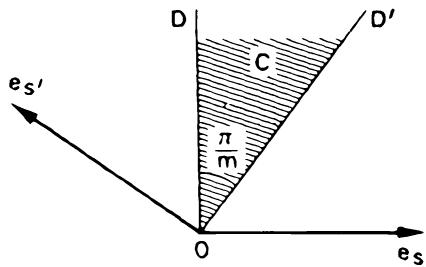
\includegraphics[keepaspectratio]{images/part001_dfbe6528.jpg}}\\
Fig. 2

\subsection{FUNDAMENTAL DOMAIN OF W IN THE UNION OF THE CHAMBERS}

We retain the notation of no. 4. For \(s \in S\) , denote by \(H_s\) the hyperplane of \(E^*\) orthogonal to \(e_s\) , by \(\overline{A_s}\) the set of \(x^* \in E^*\) such that \(\langle x^*, e_s \rangle \geqslant 0\) and by \(\overline{C}\) the intersection of the \(\overline{A_s}\) for \(s \in S\) . For the weak topology \(\sigma(E^*, E)\) defined by the duality between \(E^*\) and \(E\) (Topological Vector Spaces, Chap. II, §6, no. 2), the \(\overline{A_s}\) are closed half-spaces and \(\overline{C}\) is a closed convex cone. Moreover, \(\overline{C}\) is the closure of C; indeed, if \(x^* \in \overline{C}\) and \(y^* \in C\) , then \(x^* + ty^* \in C\) for every real number \(t > 0\) and \(x^* = \lim_{t \to 0} (x^* + ty^*)\) .

For \(X\subset S\) ,put

\[
C _ {X} = \left(\bigcap_ {s \in X} H _ {s}\right) \cap \left(\bigcap_ {s \in S - X} A _ {s}\right).
\]

We have \(C_X \subset \overline{C}\) , \(C_{\varnothing} = C\) and \(C_S = \{0\}\) . The sets \(C_X\) , for \(X \in B(S)\) , form a partition of \(\overline{C}\) .

On the other hand, recall (Chap. IV, §1, no. 8) that \(\mathbf{W}_{\mathbf{X}}\) denotes the subgroup of \(\mathbf{W}\) generated by \(\mathbf{X}\) . Clearly \(w(x^{*}) = x^{*}\) for \(w \in \mathbf{W}_{\mathbf{X}}\) and \(x^{*} \in \mathbf{C}_{\mathbf{X}}\) .

PROPOSITION 5. Let \(X, X' \subset S\) and \(w, w' \in W\) . If \(w(C_X) \cap w'(C_{X'}) \neq \emptyset\) , then \(X = X'\) , \(wW_X = w'W_{X'}\) and \(w(C_X) = w'(C_{X'})\) .

We are reduced immediately to the case \(w' = 1\) . The proof is by induction on the length \(n\) of \(w\) . If \(n = 0\) , the assertion is clear. If \(l(w) > 0\) , there exists \(s \in S\) such that \(l(sw) = l(w) - 1\) and then (cf.~the end of no. 4) \(w(C) \subset s(A_s)\) , hence \(w(\overline{C}) \subset s(\overline{A_s})\) . Since \(\overline{C} \subset \overline{A_s}\) , it follows that

\[
\overline {{{\mathrm{C}}}} \cap w (\overline {{{\mathrm{C}}}}) \subset \mathrm{H} _ {s}.
\]

Then \(s(x^{*}) = x^{*}\) for all \(x^{*} \in \overline{\mathrm{C}} \cap w(\overline{\mathrm{C}})\) , and a fortiori for all

\[
x ^ {*} \in \mathrm{C} _ {\mathrm{X} ^ {\prime}} \cap w (\mathrm{C} _ {\mathrm{X}}).
\]

Consequently, the relation \(C_{X'} \cap w(C_X) \neq \varnothing\) implies on the one hand that \(C_{X'} \cap H_s \neq \varnothing\) , and hence that \(s \in X'\) , and on the other hand that \(C_{X'} \cap sw(C_X) \neq \varnothing\) . The induction hypothesis then implies that \(X = X'\) and \(swW_X = W_{X'} = W_X\) , so \(sw \in W_X\) and \(w \in W_X\) since \(s \in W_X\) . It follows that \(wW_X = W_{X'}\) and that \(w(C_X) = C_X = C_{X'}\) .

COROLLARY. Let X be a subset of S and \(x^{*}\) an element of \(C_{X}\) . The stabiliser of \(x^{*}\) in W is \(W_{X}\) .

Now let U be the union of the \(w(\overline{\mathbf{C}})\) for \(w \in W\) , and let F be the set of subsets of U of the form \(w(\mathrm{C}_{X})\) , with \(X \subset S\) and \(w \in W\) . By the above, F is a partition of U.

PROPOSITION 6. (i) The cone U is convex.

\begin{enumerate}
\def\labelenumi{(\roman{enumi})}
\setcounter{enumi}{1}
\item
  Every closed segment contained in U meets only finitely many elements of \(\mathfrak{F}\) .
\item
  The cone \(\overline{\mathbf{C}}\) is a fundamental domain for the action of W on U.
\end{enumerate}

To prove (iii), it is enough to show that, if \(x^{*}, y^{*} \in \overline{\mathbb{C}}\) and \(w \in \mathbb{W}\) are such that \(w(x^{*}) = y^{*}\) , then \(x^{*} = y^{*}\) . Now there exist two subsets \(\mathbf{X}\) and \(\mathbf{Y}\) of \(\mathbf{S}\) such that \(x^{*} \in \mathrm{C}_{\mathbf{X}}\) and \(y^{*} \in \mathrm{C}_{\mathbf{Y}}\) ; we have \(w(\mathrm{C}_{\mathbf{X}}) \cap \mathrm{C}_{\mathbf{Y}} \neq \emptyset\) , and Prop. 5 shows that \(\mathbf{X} = \mathbf{Y}\) and \(w \in \mathrm{W}_{\mathbf{X}}\) , which implies that \(x^{*} = y^{*}\) .

Now let \(x^{*}, y^{*} \in \mathrm{U}\) ; we shall show that the segment \([x^{*}y^{*}]\) is covered by finitely many elements of \(\mathfrak{F}\) , which will establish both (i) and (ii). By transforming \(x^{*}\) and \(y^{*}\) by the same element of \(\mathrm{W}\) , we can assume that \(x^{*} \in \overline{\mathrm{C}}\) . Let \(w \in \mathrm{W}\) be such that \(y^{*} \in w(\overline{\mathrm{C}})\) . We argue by induction on the length of \(w\) . For \(s \in \mathrm{S}\) , the relation \(w(\overline{\mathrm{C}}) \not\subset \overline{\mathrm{A}_{s}}\) is equivalent to \(w(\mathrm{C}) \notin \mathrm{A}_{s}\) and hence to \(l(sw) < l(w)\) (cf.~no. 4). Prop. 7 of no. 8 of Chap. IV, §1 now implies that there exist only finitely many \(s \in \mathrm{S}\) such that \(w(\overline{\mathrm{C}}) \not\subset \overline{\mathrm{A}_{s}}\) . The set \(T\) of \(s \in S\) such that \(\langle y^{*}, e_{s} \rangle < 0\) is thus finite. On the other hand, the intersection \(\overline{\mathrm{C}} \cap [x^{*}y^{*}]\) is a closed segment \([x^{*}z^{*}]\) . If \(z^{*} = y^{*}\) , that is if \(y^{*} \in \overline{\mathrm{C}}\) , there exist subsets \(X\) and \(Y\) of \(S\) such that \(x^{*} \in C_{X}\) and \(y^{*} \in C_{Y}\) . The open segment \(|x^{*}y^{*}|\) is then contained in \(C_{X \cap Y}\) , so \([x^{*}y^{*}] \subset C_{X} \cup C_{Y} \cup C_{X \cap Y}\) . If \(z^{*} \neq y^{*}\) , there exists an \(s \in T\) such that \(z^{*} \in H_{s}\) . Then \(w(C) \not\subset A_{s}\) and \(l(sw) < l(w)\) . The induction hypothesis thus implies that the segment \([z^{*}y^{*}] = s([z^{*}(s(y^{*}))])\) is covered by a finite number of elements of \(\mathfrak{F}\) , and hence so is

\[
\left[ x ^ {*} y ^ {*} \right] = \left[ x ^ {*} z ^ {*} \right] \cup \left[ z ^ {*} y ^ {*} \right]
\]

since \([x^{*}z^{*}]\subset \overline{\mathbf{C}}.\)

\subsection{IRREDUCIBILITY OF THE GEOMETRIC REPRESENTATION OF A COXETER GROUP}

We retain the notation of the preceding nos., and assume that S is finite.

PROPOSITION 7. Assume that (W,S) is irreducible (Chap. IV, §1, no. 9). Let \(\mathbf{E}^0\) be the subspace of E orthogonal to E with respect to \(\mathbf{B}_{\mathbf{M}}\) . The group W acts trivially on \(\mathbf{E}^0\) , and every subspace of E distinct from E and stable under W is contained in \(\mathbf{E}^0\) .

If \(x \in \mathrm{E}^0\) , then \(\sigma_s(x) = x - 2\mathrm{B}_{\mathrm{M}}(e_s, x)e_s = x\) for all \(s \in \mathrm{S}\) . Since \(\mathrm{W}\) is generated by \(\mathrm{S}\) , it follows that \(\mathrm{W}\) acts trivially on \(\mathrm{E}^0\) .

Let \(E'\) be a subspace of \(E\) stable under \(W\) . Let \(s, s' \in S\) be two elements that are linked in the graph \(\Gamma\) of \((W, S)\) (Chap. IV, §1, no. 9); recall that this means that \(m(s, s') \geqslant 3\) . Suppose that \(e_s \in E'\) . Then \(\sigma_{s'}(e_s) \in E'\) and since the coefficient of \(e_{s'}\) in \(\sigma_{s'}(e_s)\) is non-zero, we have \(e_{s'} \in E'\) . Since \(\Gamma\) is connected, it follows that, if \(E'\) contains one of the \(e_s\) it contains them all and coincides with \(E\) . Except in this case, it follows from Prop. 3 of §2, no. 2 that, for all \(s \in S\) , \(E'\) is contained in the hyperplane \(H_s\) orthogonal to \(e_s\) . Since the intersection of the \(H_s\) is equal to \(E^0\) , this proves the proposition.

COROLLARY. Assume that (W, S) is irreducible. Then:

\begin{enumerate}
\def\labelenumi{\alph{enumi})}
\item
  If \(\mathrm{B_M}\) is non-degenerate, the W-module E is absolutely simple.
\item
  If \(\mathrm{B_M}\) is degenerate, the W-module E is not semi-simple.
\end{enumerate}

In case \(a\) ), Prop. 7 shows that \(E\) is simple, hence also absolutely simple (§ 2, no. 1, Prop. 1).

In case \(b\) ), \(\mathrm{E}^0 \neq 0\) , \(\mathrm{E} \neq \mathrm{E}^0\) (since \(\mathrm{B}_{\mathrm{M}} \neq 0\) ), and Prop. 7 shows that \(\mathrm{E}^0\) has no complement stable under W; thus, the W-module E is not semi-simple.

\subsection{FINITENESS CRITERION}

We retain the notation of the preceding nos., and assume that S is finite.

THEOREM 2. The following properties are equivalent:

\begin{enumerate}
\def\labelenumi{(\arabic{enumi})}
\item
  W is finite.
\item
  The form \(B_{M}\) is positive and non-degenerate.
\item
  \(\Longrightarrow\) (2). Let \(S = \bigcup_{i} S_{i}\) be the decomposition of \(S\) into connected components (Chap. IV, § 1, no. 9), and let \(W = \prod_{i} W_{i}\) be the corresponding decomposition of \(W\) . The space \(E\) can be identified with the direct sum of the spaces \(E_{i} = R^{S_{i}}\) , and \(B_{M}\) can be identified with the direct sum of the corresponding forms \(B_{M_{i}}\) . We are thus reduced to the case when \((W, S)\) is irreducible. Since \(W\) is assumed to be finite, \(E\) is a semi-simple \(W\) -module (Appendix, Prop. 2). By the Cor. to Prop. 5, it follows that \(E\) is absolutely simple. Let \(B'\) be a positive non-degenerate form on \(E\) , and let \(B''\) be the sum of its transforms under \(W\) . Since \(B''\) is invariant under \(W\) , it is proportional to \(B_{M}\) ( \(\S 2\) , no. 1, Prop. 1); since \(B_{M}(e_{s}, e_{s}) = 1\) for all \(s \in S\) , the coefficient of proportionality is \(>0\) , and since \(B''\) is positive so is \(B_{M}\) , which proves (2).
\item
  \(\Longrightarrow\) (1). If \(B_{M}\) is positive non-degenerate, the orthogonal group \(\mathbf{O}(B_{M})\) is compact (Integration, Chap. VII, §3, no. 1). Since \(\sigma(W)\) is a discrete subgroup of \(\mathbf{O}(B_{M})\) (Cor. 3 of Th. 1), it follows that \(\sigma(W)\) is finite, hence so is W. Q.E.D.
\end{enumerate}

The following result has been established in the course of the proof:

COROLLARY. If \((\mathrm{W},\mathrm{S})\) is irreducible and finite, \(\mathbf{E}\) is an absolutely simple W-module.

The finiteness criterion provided by Th. 2 permits the classification of all finite Coxeter groups (cf.~Chap. VI, §4). We restrict ourselves here to the following preliminary result:

PROPOSITION 8. If W is finite, the graph of (W, S) is a forest (Chap. IV, Appendix).

If not, this graph would contain a circuit \((s_{1},\ldots,s_{n})\) , \(n\geqslant3\) . Putting \(m_{i}=m(s_{1},s_{i+1})\) , \(1\leqslant i<n\) , and \(m_{n}=m(s_{n},s_{1})\) , this means that \(m_{i}\geqslant3\) for all i. Let

\[
x = e _ {s _ {1}} + \dots + e _ {s _ {n}}.
\]

Then \(\mathrm{B_M}(x,x) = n + 2\sum_{i < j}\mathrm{B_M}(e_{s_i},e_{s_j})\) . Now

\[
\mathrm{B} _ {\mathrm{M}} (e _ {s _ {i}}, e _ {s _ {i + 1}}) = - \cos \frac {\pi}{m _ {i}} \leqslant - \cos \frac {\pi}{3} \leqslant - \frac {1}{2},
\]

and similarly for \(\mathrm{B}_{\mathbb{M}}(e_{s_n}, e_{s_i})\) . Since the other terms in the sum are \(\leqslant 0\) , we obtain

\[
\mathrm{B} _ {\mathrm{M}} (x, x) \leqslant n - n = 0,
\]

contrary to the fact that \(B_{M}\) is positive non-degenerate.

COROLLARY. If (W, S) is irreducible and finite, its graph is a tree.

Indeed, a connected forest is a tree.

Comparison with the results of §3.

First of all let \((W,S)\) be a finite Coxeter group. Denote by \((x|y)\) the form \(\mathrm{B}_{\mathbf{M}}(x,y)\) ; by Th. 2, this is a scalar product on E. For all \(s \in S\) , let \(H_{s}\) be the hyperplane associated to the orthogonal reflection \(\sigma_{s}\) , and let \(\mathfrak{H}\) be the family of hyperplanes \(w(\mathrm{H}_{s})\) , for \(s \in S\) , \(w \in W\) . Let \(C_{0}\) be the set of \(x \in E\) such that \((x|e_{s}) > 0\) for all \(s \in S\) . Finally, identify W (by means of \(\sigma\) ) with a subgroup of the orthogonal group \(\mathbf{O}(\mathbf{E})\) of the space E.

PROPOSITION 9. With the preceding notations, W is the subgroup of O(E) generated by the reflections with respect to the hyperplanes of \(\mathfrak{H}\) . It is an essential group (§3, no. 7) and C0 is a chamber of E relative to \(\mathfrak{H}\) .

The first assertion is trivial. On the other hand, if \(x \in E\) is invariant under W, it is orthogonal to all the \(e_{s}\) , and hence is zero; this shows that W is essential. Finally, the isomorphism \(E \to E^{*}\) defined by \(B_{M}\) transforms \(C_{0}\) to the set C of no. 4; the property \((P_{n})\) proved there shows that, for all \(w \in W\) and all \(s \in S\) , \(w(C_0)\) does not meet \(H_s\) . It follows that \(C_0\) is contained in the complement U of the union of the hyperplanes of \(\mathfrak{H}\) , and since \(C_0\) is connected, open and closed in U, it is a chamber of E relative to \(\mathfrak{H}\) . Q.E.D.

We can apply to W and \(C_{0}\) all the properties proved in §3. In particular, \(\overline{C_{0}}\) is a fundamental domain for the action of W on E (in other words, the cone U defined in no. 6 is equal to the whole of E).

Conversely, let E be a finite dimensional real vector space, provided with a scalar product \((x|y)\) and let W be an essential finite group of displacements of E leaving 0 fixed; assume that W is generated by reflections. Let \(C_{0}\) be a chamber of E with respect to W (cf.~§3), and let S be the set of orthogonal reflections relative to the walls of \(C_{0}\) . Then (W, S) is a finite Coxeter system (§3, no. 2, Th. 1). Moreover, if \(s \in S\) , denote by \(H_{s}\) the wall of \(C_{0}\) corresponding to s, and denote by \(e_{s}\) the unit vector orthogonal to \(H_{s}\) and on the same side of \(H_{s}\) as \(C_{0}\) . If \((m(s, s'))\) denotes the Coxeter matrix of (W, S), Props. 3 and 7 of §3 show that

\[
(e _ {s} | e _ {s ^ {\prime}}) = - \cos (\pi / m (s, s ^ {\prime}))
\]

and that the \(e_{s}\) form a basis of E. The natural representation of W on E can thus be identified with the representation \(\sigma\) of no. 3.

\subsection{\texorpdfstring{CASE IN WHICH \(\mathbf{B}_{\mathrm{M}}\) IS POSITIVE AND DEGENERATE}{CASE IN WHICH B\_M IS POSITIVE AND DEGENERATE}}

In this number, we assume that S is finite, that \((W, S)\) is irreducible, and that the form \(B_{M}\) is positive and degenerate.

Lemma 2. The orthogonal complement \(\mathbf{E}^0\) of \(\mathbf{E}\) for \(\mathbf{B}_{\mathbf{M}}\) is of dimension 1; it is generated by an element \(v = \sum_{s\in S}v_s e_s\) with \(v_{s} > 0\) for all \(s\) .

This follows from Lemma 4 of §3, no. 5, applied to the matrix with entries \(\mathrm{B}_{\mathbb{M}}(e_s, e_{s'})\) .

Let \(v = \sum_{s} v_s e_s\) be the vector satisfying the conditions of Lemma 2 and such that \(\sum_{s} v_s = 1\) , and let A be the affine hyperplane of \(E^*\) consisting of the \(y^* \in E^*\) such that \(\langle v, y^* \rangle = 1\) . If T denotes the orthogonal complement of \(v\) in \(E^*\) , A has a natural structure of an affine space with space of translations T. Moreover, the form \(B_M\) defines by passage to the quotient a non-degenerate scalar product on \(E/E^0\) , hence also on its dual T; this gives a euclidean structure on the affine space A (Algebra, Chap. IX, §6, no. 6).

Let G be the subgroup of \(\mathbf{GL}(\mathbf{E})\) consisting of the automorphisms leaving v and \(B_{M}\) invariant; if \(g \in G\) , the contragredient map \({}^{t}g^{-1}\) leaves A and T stable, and defines by restriction to A a displacement \(i(g)\) of A (cf.~§3). It is immediate that this gives an isomorphism from G to the group of displacements of A. Moreover, the stabiliser \(G_{a}\) of a point a of A can be identified with the orthogonal group of the Hilbert space T and is thus compact. On the other hand, G is a locally compact group countable at infinity and A is a Baire space: it follows (Integration, Chap. VII, Appendix, Lemma 2) that the map \(\psi : g \mapsto g(a)\) defines a homeomorphism from \(G/G_a\) to A. Thus G acts properly on A (General Topology, Chap. III, §4, no. 2, Prop. 5). Since W is a subgroup of G, it can be identified with a group of displacements of A. We are going to show that this group satisfies the assumptions of §3. More precisely:

PROPOSITION 10. The group W provided with the discrete topology acts properly on A; it is generated by orthogonal reflections; it is infinite, irreducible and essential (§3, no. 7). The intersection C ∩ A is a chamber of A for W. If L\_s denotes the hyperplane of A formed by the intersection of A with the hyperplane of E* orthogonal to e\_s, the L\_s for s ∈ S are the walls of C ∩ A. If ε\_s is the unit vector of T orthogonal to L\_s on the same side of L\_s as C ∩ A, then (ε\_s\textbar ε\_t) = -cos(π/m(s,t)) (for s,t ∈ S) and the Coxeter matrix of W (§3, no. 4) is identified with M.

By Cor. 3 of Th. 1, W is discrete in \(\mathbf{GL}(\mathbf{E})\) , and hence in \(\mathbf{G}\) , and acts properly on A. Let \(s \in S\) . Since \(\operatorname{Card} S \geqslant 2\) , the hyperplane of \(\mathbf{E}^*\) orthogonal to \(e_s\) is not orthogonal to \(v\) and its intersection \(\mathbf{L}_s\) with A is indeed a hyperplane. The displacement corresponding to \(s\) is thus a displacement of order 2 leaving fixed all the points of \(\mathbf{L}_s\) : it is necessarily the orthogonal reflection associated to \(\mathbf{L}_s\) . It follows that W is generated by orthogonal reflections. Th. 2 now shows that it is infinite and Prop. 7 that it is essential and irreducible.

Since C is an open simplicial cone, whose walls are the hyperplanes with equations \(\langle x^{*}, e_{s} \rangle = 0\) (for \(s \in S\) ), the intersection \(C \cap A\) is a convex, hence connected, open and closed subset of the complement of the union of the \(L_{s}\) in A. Moreover, \(C \cap A\) is non-empty, for if \(x^{*} \in C\) we have \(\langle x^{*}, v \rangle = \sum_{s} v_{s} \langle x^{*}, e_{s} \rangle > 0\) and \(\langle x^{*}, v \rangle^{-1} x^{*} \in C \cap A\) . It follows that \(C \cap A\) is a chamber of A relative to the system of the \(L_{s}\) . Moreover, \(w(C \cap A) \cap L_{s} = \varnothing\) for all \(w \in W\) (cf.~no. 4, property \((\mathrm{P}_{n})\) ) and it follows that \(C \cap A\) is a chamber of A relative to the system consisting of the transforms of the \(L_{s}\) by the elements of W; by the Cor. of Th. 1 of §3, no. 2, it follows that \(C \cap A\) is a chamber of A relative to W.

Let \(a_{s}^{*}\) be the vertex of the simplex \(C \cap A\) not in \(L_{s}\) . We have

\[
\left\langle a _ {s} ^ {*}, e _ {t} \right\rangle = 0
\]

for \(s,t\in \mathrm{S}\) and \(s\neq t\) , and

\[
\langle a _ {s} ^ {*}, e _ {s} \rangle = v _ {s} ^ {- 1} \langle a _ {s} ^ {*}, v \rangle = v _ {s} ^ {- 1}.
\]

Let \(\varepsilon_{s}\) be the vector in T defined by the relations:

\[
\left(\varepsilon_ {s} \mid a _ {s} ^ {*} - a _ {t} ^ {*}\right) = v _ {s} ^ {- 1} \text {for} t \in S, t \neq s.
\]

The vector \(\varepsilon_{s}\) is orthogonal to \(L_{s}\) and is on the same side of the hyperplane \(L_{s}\) as \(C \cap A\) . Moreover

\[
\left(\varepsilon_ {s} \mid a _ {s} ^ {*} - a _ {t} ^ {*}\right) = \left\langle e _ {s}, a _ {s} ^ {*} - a _ {t} ^ {*} \right\rangle \text {for all} s, t \in S
\]

which shows that \(\varepsilon_{s}\) is the image of the class of \(e_{s}\) under the isomorphism from \(E/E^{0}\) to T given by the quadratic form \(B_{M}\) . It follows that

\[
(\varepsilon_ {s} | \varepsilon_ {t}) = \mathrm{B} _ {\mathrm{M}} (e _ {s}, e _ {t}).
\]

Consequently \(\varepsilon_{s}\) is a unit vector and the last assertion of Prop. 10 is proved.

The euclidean affine space A provided with the group W is called the space associated to the Coxeter matrix M and we denote it by \(A_{M}\) .

Proposition 10 admits a converse:

PROPOSITION 11. Let W be a group of displacements of a euclidean affine space A, satisfying the assumptions of §3. Assume that W is infinite, essential and irreducible. Then the form \(B_{M}\) attached to the Coxeter matrix M of W is positive degenerate and there exists a unique isomorphism from the affine space \(A_{M}\) associated to M to A, commuting with the action of W. This isomorphism transforms the scalar product of \(A_{M}\) into a multiple of the scalar product of A.

Let \(C_0\) be a chamber of A and let S be the set of orthogonal reflections with respect to the walls of \(C_0\) . If \(\eta_s\) denotes the unit vector orthogonal to the hyperplane \(N_s\) associated to the reflection s and on the same side of \(N_s\) as \(C_0\) (§3, Prop. 3), the form \(B_M\) is such that \(B_M(e_s, e_t) = (\eta_s | \eta_t)\) for \(s, t \in S\) . It is thus positive. Since the \(\eta_s\) are linearly dependent (§3, no. 9, Prop. 8), it is degenerate.

We can thus apply the preceding constructions to M. With the same notation as above, \((\varepsilon_{s}|\varepsilon_{t}) = (\eta_{s}|\eta_{t})\) and there exists a unique isomorphism \(\varphi\) of Hilbert spaces from T to the space of translations of A such that \(\varphi(\varepsilon_{s}) = \eta_{s}\) . Let a and b be two distinct vertices of \(C_{0}\) and \(s_{0}\) the reflection in S such that \(a \notin N_{s_{0}}\) . Put \(\lambda = (\eta_{s}|a - b)\) and let \(\psi\) be the affine bijection from \(A_{M}\) to A defined by

\[
\psi \left(a _ {s _ {0}} + x\right) = a + v _ {s _ {0}} \lambda \varphi (x) \text {for} x \in \mathrm{T}.
\]

It is then immediate that \(\psi(\mathrm{L}_{s}) = \mathrm{N}_{s}\) for all \(s \in S\) and that \(\psi\) transforms the scalar product of \(A_{M}\) into a multiple of that on A. It follows at once that \(\psi\) commutes with the action of W. Finally, the uniqueness of \(\psi\) is evident, for \(a_{s}\) for example is the unique point of \(A_{M}\) invariant under the reflections \(t \in S, t \neq s\) .

\section{INVARIANTS IN THE SYMMETRIC ALGEBRA}

\subsection{POINCARÉ SERIES OF GRADED ALGEBRAS}

Let K be a commutative ring with unit element, not reduced to 0. Let M be a graded K-module of type Z, and \(M_{n}\) the set of homogeneous elements of M of degree n.~Assume that each \(M_{n}\) is free and of finite type. Then the rank \(\operatorname{rk}_{\mathbf{K}}(\mathbf{M}_{n})\) is defined for all n (Commutative Algebra, Chap. II, §5, no. 3).

DEFINITION 1. If there exists \(n_0 \in \mathbf{Z}\) such that \(M_n = 0\) for \(n \leqslant n_0\) , the formal series \(\sum_{n \geqslant n_0} \mathrm{rk}_K(M_n) T^n\) , which is an element of \(\mathbf{Q}((T))\) , is called the Poincaré series of \(M\) and denoted by \(P_M(T)\) .

Let \(M'\) be another graded K-module of type Z, and \((M_n')_{n \in \mathbf{Z}}\) its grading. Assume that \(M_n'\) is zero for n less than a certain number. Then

\[
\mathrm{P} _ {\mathrm{M} \oplus \mathrm{M} ^ {\prime}} (\mathrm{T}) = \mathrm{P} _ {\mathrm{M}} (\mathrm{T}) + \mathrm{P} _ {\mathrm{M} ^ {\prime}} (\mathrm{T})\tag{1}
\]

and, if \(\mathbf{M} \otimes_{\mathbf{K}} \mathbf{M}'\) is provided with the total grading (Algebra, Chap. II, §11, no. 5),

\[
\mathrm{P} _ {\mathrm{M} \otimes \mathrm{M} ^ {\prime}} (\mathrm{T}) = \mathrm{P} _ {\mathrm{M}} (\mathrm{T}) \mathrm{P} _ {\mathrm{M} ^ {\prime}} (\mathrm{T}).\tag{2}
\]

PROPOSITION 1. Let \(S = \bigoplus_{n \geqslant 0} S_n\) be a commutative graded K-algebra with a system of generators \((x_1, x_2, \ldots, x_m)\) consisting of homogeneous and algebraically independent elements. Let \(d_i\) be the degree of \(x_i\) , and assume that \(d_i > 0\) for all \(i\) . Then the \(S_n\) are free and of finite rank over \(K\) , and

\[
\mathrm{P} _ {\mathrm{S}} (\mathrm{T}) = \prod_ {i = 1} ^ {m} (1 - \mathrm{T} ^ {d _ {i}}) ^ {- 1}.\tag{3}
\]

Indeed, S can be identified with the tensor product \(K[x_{1}] \otimes \cdots \otimes K[x_{m}]\) , provided with the total grading. The Poincaré series of \(K[x_{i}]\) is

\[
\sum_ {n \geqslant 0} \mathrm{T} ^ {n d _ {i}} = (1 - \mathrm{T} ^ {d _ {i}}) ^ {- 1},
\]

and it suffices to apply (2).

Under the assumptions of Prop. 1, we shall say that S is a graded polynomial algebra over K.

COROLLARY. The degrees \(d_{i}\) are determined up to order by S.

Indeed, the inverse of \(\mathrm{P}_{\mathrm{S}}(\mathrm{T})\) is the polynomial \(\mathrm{N}(\mathrm{T}) = \prod_{i=1}(1 - \mathrm{T}^{d_i})\) , which is thus uniquely determined. If q is an integer \(\geqslant 1\) and if \(\zeta \in C\) is a primitive qth root of unity, the multiplicity of the root \(\zeta\) of \(\mathrm{N}(\mathrm{T})\) is equal to the number of \(d_{i}\) that are multiples of q. This number is zero for q sufficiently large. The number of \(d_{i}\) equal to q is thus determined uniquely by descending induction.

The integers \(d_{i}\) are called the characteristic degrees of S. The number of them is equal to the transcendence degree of S over K when K is a field; we shall also call it the transcendence degree of S over K in the general case. It is the multiplicity of the root 1 of the polynomial N(T).

Let \(S = \bigoplus_{n \geqslant 0} S_n\) be a commutative graded K-algebra, and \(R = \bigoplus_{n \geqslant 0} R_n\) a graded subalgebra of S. Assume that each \(R_n\) is free and of finite type, and that the R-module S admits a finite basis consisting of homogeneous elements \(z_1, z_2, \ldots, z_N\) of degrees \(f_1, f_2, \ldots, f_N\) . Then, if M denotes the graded K-module \(\sum_{j=1}^{N} Kz_j\) , the graded K-module S is isomorphic to \(R \otimes_K M\) , so each \(S_n\) is free and of finite type and

\[
P _ {S} (T) = P _ {M} (T) P _ {R} (T) = \left(\sum_ {j = 1} ^ {N} T ^ {f _ {j}}\right) P _ {R} (T).\tag{4}
\]

PROPOSITION 2. Retain the preceding notation and assume that \(S\) and \(R\) are graded polynomial algebras.

\begin{enumerate}
\def\labelenumi{(\roman{enumi})}
\item
  R and S have the same transcendence degree \(r\) over \(K\) .
\item
  Let \(p_1, \ldots, p_r\) (resp. \(q_1, \ldots, q_r\) ) be the characteristic degrees of \(S\) (resp. \(R\) ). Then
\end{enumerate}

\[
\prod_ {i = 1} ^ {r} \left(1 - \mathrm{T} ^ {q _ {i}}\right) = \left(\sum_ {j = 1} ^ {\mathrm{N}} \mathrm{T} ^ {f _ {j}}\right) \prod_ {i = 1} ^ {r} \left(1 - \mathrm{T} ^ {p _ {i}}\right).
\]

\begin{enumerate}
\def\labelenumi{(\roman{enumi})}
\setcounter{enumi}{2}
\tightlist
\item
  \(Np_{1}p_{2}\ldots p_{r}=q_{1}q_{2}\ldots q_{r}.\)
\end{enumerate}

Formula (4) shows first of all that the multiplicity of the root 1 is the same in the polynomials \(\mathrm{P}_{\mathrm{S}}(\mathrm{T})^{-1}\) and \(\mathrm{P}_{\mathrm{R}}(\mathrm{T})^{-1}\) and, taking (3) into account, proves both (i) and (ii).

It follows from (ii) that

\[
\prod_ {i = 1} ^ {r} \left(1 + \mathrm{T} + \mathrm{T} ^ {2} + \dots + \mathrm{T} ^ {q _ {i} - 1}\right) = \left(\sum_ {j = 1} ^ {\mathrm{N}} \mathrm{T} ^ {f _ {j}}\right) \prod_ {i = 1} ^ {r} \left(1 + \mathrm{T} + \mathrm{T} ^ {2} + \dots + \mathrm{T} ^ {p _ {i} - 1}\right).
\]

Putting \(\mathrm{T} = 1\) in this relation gives (iii).

Remark. Let \(S = K[X_1, \ldots, X_n]\) be a graded polynomial algebra over \(K\) , \(d_i\) the degree of \(X_i\) and \(F(X_1, \ldots, X_n)\) a homogeneous element of degree \(m\) of \(S\) . Then

\[
\sum_ {i = 1} ^ {n} d _ {i} X _ {i} \frac {\partial F}{\partial X _ {i}} = m F.\tag{5}
\]

Indeed, it is immediate that the K-linear map D from S to S that transforms every homogeneous element z of degree p into pz is a derivation of S. Thus

\[
m \mathrm{F} (\mathrm{X} _ {1}, \dots , \mathrm{X} _ {n}) = \mathrm{D} (\mathrm{F} (\mathrm{X} _ {1}, \dots , \mathrm{X} _ {n})) = \sum_ {i = 1} ^ {n} \mathrm{D} (\mathrm{X} _ {i}) \frac {\partial \mathrm{F}}{\partial \mathrm{X} _ {i}} = \sum_ {i = 1} ^ {n} d _ {i} \mathrm{X} _ {i} \frac {\partial \mathrm{F}}{\partial \mathrm{X} _ {i}}.
\]

\subsection{INVARIANTS OF A FINITE LINEAR GROUP: MODULAR PROPERTIES}

Let K be a commutative ring, V a K-module, and G a group acting on V. We know that every automorphism of V extends uniquely to an automorphism of the symmetric algebra \(S = \mathbf{S}(V)\) , and thus G acts on this algebra. If \(x \in S\) and \(g \in G\) , we denote by \(g_{S}.x\) the transform of x by g. Let R be the subalgebra \(S^{G}\) of S formed by the elements invariant under G.

Assume that G is finite, V is of finite type, and K is noetherian. Then S is an R-module of finite type, and R is a K-algebra of finite type (Commutative Algebra, Chap. V, §1, no. 9, Th. 2). Assume that S is integral and let N be its field of fractions. The field of fractions L of R is the set of elements of N invariant under G (loc. cit., Cor. of Prop. 23), so N is a Galois extension of L. Every element of N can be written z/t with \(z \in S\) and \(t \in R\) (loc. cit., Prop. 23). By Algebra, Chap. II, §7, no. 10, Cor. 3 of Prop. 26, the rank of the R-module S is {[}N : L{]}. Assume that G acts faithfully on V. The Galois group of N over L can then be identified with G, so {[}N : L{]} = Card G; thus

\[
\operatorname{rk} _ {\mathsf {R}} (\mathrm{S}) = [ \mathrm{N}: \mathrm{L} ] = \operatorname{Card} (\mathrm{G}).\tag{6}
\]

For any graded algebra \(A = A_{0} \oplus A_{1} \oplus \cdots \oplus A_{n} \oplus \cdots\) , denote by \(A_{+}\) the ideal \(\bigoplus_{n > 0} A_{n}\) .

THEOREM 1. Let K be a commutative field, V a finite dimensional vector space over K, S = S(V) the symmetric algebra of V, G a finite group of automorphisms of V, and R the graded subalgebra of S consisting of the elements invariant under G. Assume that G is generated by pseudo-reflections (§2, no. 1) and that q = Card(G) is coprime to the characteristic of K. Then the R-module S has a basis consisting of q homogeneous elements.

\begin{enumerate}
\def\labelenumi{\alph{enumi})}
\item
  Since every submodule of \(S/(R_{+}S)\) is free over \(R_0 = K\) , it is enough to show (in view of Algebra, Chap. II, §11, no. 4, Prop. 7) that the canonical homomorphism from \(R_{+} \otimes_{R} S\) to \(S\) is injective. For any R-module \(E\) , denote by \(T(E)\) the R-module \(\text{Ker}(R_{+} \otimes_{R} E \to E)\) (*in other words, \(T(E) = \text{Tor}_{1}^{R}(R/R_{+}, E)_*\) ). If \(E, E'\) are two R-modules and \(u\) is a homomorphism from \(E\) to \(E'\) , the homomorphism \(1 \otimes u\) from \(R_{+} \otimes E\) to \(R_{+} \otimes E'\) defines by restriction to \(T(E)\) a homomorphism from \(T(E)\) to \(T(E')\) that we denote by \(T(u)\) . If \(u'\) is a homomorphism from \(E'\) to an R-module \(E''\) , we have \(T(u' \circ u) = T(u') \circ T(u)\) . Thus, if G acts R-linearly on \(E\) , then G acts on \(T(E)\) .
\item
  The group G acts R-linearly on S, and hence also on T(S). Moreover, T(S) has a natural structure of graded S-module. We show first that, if \(g \in G\) , then g transforms every element x of T(S) into an element congruent to x modulo \(S_{1}T(S)\) . It is enough to do this when g is a pseudo-reflection. Then there exists a non-zero vector v in V such that \(g(x) - x \in Kv\) for all \(x \in V\) . Since V generates S, it follows that \(g_{S}\) acts trivially on S/Sv. Thus, for any \(y \in S\) , there exists an element \(h(y)\) in S such that
\end{enumerate}

\[
g _ {\mathrm{S}} (y) - y = h (y) v.
\]

Since S is integral and v is non-zero, this element is determined uniquely by y; it is immediate that h is an endomorphism of degree -1 of the R-module S. Thus, \(g_{S} - 1_{S} = m_{v} \circ h\) , where \(m_{v}\) denotes the homothety with ratio v in S. Hence,

\[
\mathrm{T} (g _ {\mathrm{S}}) - 1 _ {\mathrm{T(S)}} = \mathrm{T} (g _ {\mathrm{S}} - 1 _ {\mathrm{S}}) = \mathrm{T} (m _ {v}) \circ \mathrm{T} (h),
\]

the image of which is contained in \(vT(S)\) , proving our assertion.

\begin{enumerate}
\def\labelenumi{\alph{enumi})}
\setcounter{enumi}{2}
\tightlist
\item
  We show that any element of \(T(S)\) invariant under G is zero. Indeed, let Q be the endomorphism of the R-module S defined by
\end{enumerate}

\[
\mathrm{Q} (y) = q ^ {- 1} \sum_ {g \in G} g _ {\mathrm{S}} (y)
\]

for all \(y \in S\) . Then \(Q(S) = R\) . We can thus write \(Q = i \circ Q'\) , where \(Q'\) is a homomorphism from the R-module S to the R-module R and i denotes the canonical injection of R into S. Thus \(T(Q) = T(i) \circ T(Q')\) and \(T(Q') = 0\) since \(T(R) = \text{Ker}(R_{+} \otimes R \to R) = 0\) . Thus

\[
0 = \mathrm{T} (\mathrm{Q}) = q ^ {- 1} \sum_ {g \in \mathrm{G}} \mathrm{T} (g _ {\mathrm{S}}).
\]

But \(q^{-1} \sum_{g \in G} T(g_S)\) leaves fixed the elements of \(T(S)\) invariant under G. These elements are therefore zero.

\begin{enumerate}
\def\labelenumi{\alph{enumi})}
\setcounter{enumi}{3}
\tightlist
\item
  Assume that \(T(S) \neq 0\) . There exists in \(T(S)\) a homogeneous element \(u \neq 0\) of minimum degree. By b), u is invariant under G. By c), u = 0. This is a contradiction, so \(T(S) = 0\) . Q.E.D.
\end{enumerate}

Remarks. 1) It follows from Algebra, Chap. II, §11, no. 4, Prop. 7 that, if \((z_{1},\ldots ,z_{q})\) is a family of homogeneous elements of S whose canonical images in \(\mathrm{S / (R_+S)}\) form a basis of \(\mathrm{S / (R_+S)}\) over K, then \((z_{1},\ldots ,z_{q})\) is a basis of S over R.

\begin{enumerate}
\def\labelenumi{\arabic{enumi})}
\setcounter{enumi}{1}
\tightlist
\item
  Let \(g\) be a pseudo-reflection of \(V\) , whose order \(n \geqslant 2\) is finite and co-prime to the characteristic of \(K\) . By Maschke's theorem (Appendix, Prop. 2), \(V\) can be decomposed as \(D \oplus H\) , where \(H\) is the hyperplane consisting of the elements of \(V\) invariant under \(g\) and \(D\) is a line on which \(g\) acts by multiplication by a primitive \(n\) th root of unity. When \(K = R\) , this is possible only when \(n = 2\) , and \(g\) is then a reflection; in this case, the groups to which Th. 1 applies are the finite Coxeter groups. (For K = C, on the other hand, Th. 1 applies to certain groups that are not Coxeter groups.) \(^{3}\)
\end{enumerate}

THEOREM 2. Retain the assumptions and notation of Theorem 1.

\begin{enumerate}
\def\labelenumi{(\roman{enumi})}
\item
  There exists a graded vector subspace of \(S\) forming a complement to \(R_{+}S\) in \(S\) and stable under \(G\) .
\item
  Let U be such a complement. The canonical homomorphism from \(U \otimes_{K} R\) to S is an isomorphism of G-modules, and the representation of G in U (resp. S) is isomorphic to the regular representation of G on K (resp. R).
\end{enumerate}

Indeed, for any integer \(n \geqslant 0\) , the K-vector spaces \(S_n\) and \((R_+S) \cap S_n\) are stable under \(G\) , and it follows from Maschke's theorem (Appendix, Prop. 2) that there exists a G-stable complement \(U_n\) of \((R_+S) \cap S_n\) in \(S_n\) . Then \(\sum_{n \geqslant 0} U_n\) is a G-stable complement of \(R_+S\) in \(S\) , hence (i).

Let U be a graded vector subspace of S forming a complement of \(R_{+}S\) in S and stable under G. By Remark 1, every basis of the K-vector space U is also a basis of the R-module S, and consequently is a basis of the field of fractions N of S over the field of fractions L of R. Thus, the L-vector space N can be identified with \(U \otimes_{K} L\) . Since U is stable under G, this identification is compatible with the action of G. The group algebra \(L[G]\) of G over L can be identified with the algebra \(K[G] \otimes_{K} L\) . The Galois extension N of L admits a normal basis (Algebra, Chap. V, §10, no. 9, Th. 6), which can be interpreted as saying that N, considered as an \(L[G]\) -module, is isomorphic to the module of the regular representation of G over L. Since U is finite dimensional over K, it follows from the Appendix, Prop. 1, that the \(K[G]\) -module U is isomorphic to the regular representation of G over K. Our assertions follow immediately from this.

\subsection{INVARIANTS OF A FINITE LINEAR GROUP: RING-THEORETIC PROPERTIES}

THEOREM 3. We retain the assumptions and notation of Th. 1. In the set of systems of generators of the ideal \(R_{+}\) of R consisting of homogeneous elements, choose a minimal element \((\alpha_{1},\ldots,\alpha_{l})\) . Let \(k_{i}\) be the degree of \(\alpha_{i}\) . Assume that the \(k_{i}\) are coprime to the characteristic exponent of K. Then \(l=\dim V\) , the \(\alpha_{i}\) generate the K-algebra R, and are algebraically independent over K. In particular, R is a graded K-algebra of polynomials of transcendence degree l over K.

The assumption made about the \(k_{i}\) is superfluous, but is irrelevant for the applications to finite Coxeter groups, since then K = R. Cf. no. 5, where we shall give another proof of Th. 3.

Th. 3 follows from Prop. 2 (i), Th. 1 and the following lemma:

Lemma 1. Let K be a commutative field, S a graded K-algebra of polynomials, and R a graded subalgebra of S of finite type such that the R-module S admits a basis \((z_{\lambda})_{\lambda \in \Lambda}\) consisting of homogeneous elements. In the set of systems of generators of the ideal \(R_{+}\) of R consisting of homogeneous elements, choose a minimal element \((\alpha_{1}, \ldots, \alpha_{s})\) . Assume that, for all i, the degree \(k_{i}\) of \(\alpha_{i}\) is coprime to the characteristic exponent p of K. Then the \(\alpha_{i}\) generate the K-algebra R and are algebraically independent over K.

By Algebra, Chap. II, § 11, no. 4, Prop. 7, the assumption made about the \(\alpha_{i}\) is equivalent to saying that they are homogeneous and that their images in the K-vector space \(R_{+}/(R_{+})^{2}\) form a basis of this space. This condition is invariant under extension of the base field; we can thus reduce to the case where the latter is perfect.

The family \((\alpha_{1},\ldots,\alpha_{s})\) generates the algebra R by Commutative Algebra, Chap. III, §1, no. 2, Prop. 1. We argue by contradiction and assume that this family is not algebraically independent over K.

\begin{enumerate}
\def\labelenumi{\arabic{enumi})}
\tightlist
\item
  We show first of all that there exist families
\end{enumerate}

\[
\left(\beta_ {i}\right) _ {1 \leqslant i \leqslant s}, \quad \left(y _ {k}\right) _ {1 \leqslant k \leqslant r}, \quad \left(d _ {i k}\right) _ {1 \leqslant i \leqslant s, 1 \leqslant k \leqslant r}
\]

of homogeneous elements of S with the following properties:

\[
\beta_ {i} \in R \text {for all} i, \text {and the} \beta_ {i} \text {are not all zero};\tag{7}
\]

\[
\deg y _ {k} > 0 \text {   for   all   } k;\tag{8}
\]

\[
\alpha_ {i} = \sum_ {k = 1} ^ {r} d _ {i k} y _ {k} \quad \text { for   all } i;\tag{9}
\]

\[
\sum_ {i = 1} ^ {s} \beta_ {i} d _ {i k} = 0 \quad \text { for   all } k.\tag{10}
\]

Let \(X_{1},\ldots,X_{s}\) be indeterminates and give \(K[X_{1},\ldots,X_{s}]\) with the graded algebra structure for which \(X_{i}\) has degree \(k_{i}\) . There exist non-zero homogeneous elements \(H(X_{1},\ldots,X_{s})\) of \(K[X_{1},\ldots,X_{s}]\) such that \(H(\alpha_{1},\ldots,\alpha_{s})=0\) ; choose H to be of minimum degree. If \(\partial H/\partial X_{i}\neq0\) , the polynomial \(\frac{\partial H}{\partial X_{i}}(\alpha_{1},\ldots,\alpha_{s})\) is a non-zero homogeneous element of R; if \(p\neq1\) , H is not of the form \(H_{1}^{p}\) with \(H_{1}\in K[X_{1},\ldots,X_{s}]\) . Take

\[
\beta_ {i} = k _ {i} \frac {\partial \mathrm{H}}{\partial \mathrm{X} _ {i}} (\alpha_ {1}, \dots , \alpha_ {s}).
\]

Since K is perfect, the polynomials \(\partial H/\partial X_{i} \in K[X_{1},\ldots,X_{s}]\) are not all zero (Algebra, Chap. V, §1, no. 3, Prop. 4); in view of the assumption made about the \(k_{i}\) , neither are the \(\beta_{i}\) .

On the other hand, S can be identified with a graded algebra of polynomials \(K[x_{1},\ldots,x_{r}]\) for appropriate indeterminates \(x_{1},\ldots,x_{r}\) with suitable degrees \(m_{i}>0\) . Let \(D_{k}\) be the partial derivative with respect to \(x_{k}\) on S. Take \(d_{ik} = k_i^{-1}\mathrm{D}_k(\alpha_i)\) . Then the equality (10) holds because its left-hand side is \(\mathrm{D}_k(\mathrm{H}(\alpha_1,\dots ,\alpha_s))\) . On the other hand, if we put \(y_{1} = m_{1}x_{1},\ldots ,y_{r} = m_{r}x_{r}\) , the equality (9) follows from the equality (5) of no. 1.

\begin{enumerate}
\def\labelenumi{\arabic{enumi})}
\setcounter{enumi}{1}
\tightlist
\item
  Let \(\mathfrak{b}\) be the ideal of \(R\) generated by the \(\beta_{i}\) ; there exists a subset \(J\) of
\end{enumerate}

\[
\mathrm{I} = \{1, 2, \dots , s \}
\]

such that \((\beta_{i})_{i\in\mathbb{J}}\) is a minimal system of generators of b. Then \(J\neq\varnothing\) since \(b\neq0\) . We shall deduce from (9) and (10) that, if \(i\in J\) , \(\alpha_{i}\) is an R-linear combination of the \(\alpha_{j}\) for \(j\neq i\) , which will contradict the minimality of \((\alpha_{1},\ldots,\alpha_{s})\) and will complete the proof.

There exist homogeneous elements \(\gamma_{ji}\) of R ( \(i \in \mathrm{J}, j \in \mathrm{I} - \mathrm{J}\) ) such that

\[
\beta_ {j} = \sum_ {i \in J} \gamma_ {j i} \beta_ {i} (j \in I - J).\tag{11}
\]

Taking (11) into account, formula (10) gives

\[
\sum_ {i \in \mathrm{J}} \beta_ {i} \left(d _ {i k} + \sum_ {j \in \mathrm{I} - \mathrm{J}} \gamma_ {j i} d _ {j k}\right) = 0.\tag{12}
\]

Put

\[
u _ {i k} = d _ {i k} + \sum_ {j \in I - J} \gamma_ {j i} d _ {j k}.\tag{13}
\]

Thus

\[
\sum_ {i \in J} \beta_ {i} u _ {i k} = 0.\tag{14}
\]

Write \(u_{ik} = \sum_{\lambda \in \Lambda} \delta_{ik\lambda} z_\lambda\) , where the \(\delta_{ik\lambda}\) belong to R. Relation (14) implies that \(\sum_{i \in J} \beta_i \delta_{ik\lambda} = 0\) for all \(k\) and \(\lambda\) . If one of the \(\delta_{ik\lambda}\) had a non-zero homogeneous component of degree 0, the preceding equality would imply that one of the \(\beta_i\) ( \(i \in J\) ) is an R-linear combination of the others, contradicting the minimality of \((\beta_i)_{i \in J}\) . Thus \(\delta_{ik\lambda} \in R_+\) and consequently \(u_{ik} \in R_+ S\) for all \(i\) and \(k\) . Thus, there exist \(u_{ikh} \in S\) such that \(u_{ik} = \sum_{h=1}^{s} u_{ikh} \alpha_h\) , in other words, by (13),

\[
d _ {i k} + \sum_ {j \in I - J} \gamma_ {j i} d _ {j k} = \sum_ {h = 1} ^ {s} u _ {i k h} \alpha_ {h}.\tag{$(15)_{ik}$}
\]

Multiply both sides of \((15)_{ik}\) by \(y_{k}\) and add for i in J fixed and \(k = 1, 2, \ldots, r\) ; in view of (9), we find that

\[
\alpha_ {i} + \sum_ {j \in I - J} \gamma_ {j i} \alpha_ {j} = \sum_ {h = 1} ^ {s} \sum_ {k = 1} ^ {r} u _ {i k h} y _ {k} \alpha_ {h}.
\]

Take the homogeneous components of degree \(k_i\) of both sides. Since \(\deg y_k > 0\) , \(\alpha_i\) is an S-linear combination of the \(\alpha_j\) for \(j \neq i\) . Since S is free over R and \(\alpha_1, \ldots, \alpha_s \in \mathrm{R}\) , it follows that \(\alpha_i\) is an R-linear combination of the \(\alpha_j\) with \(j \neq i\) (Commutative Algebra, Chap. I, §3, no. 5, Prop. 9 d)).

COROLLARY. With the assumptions and notation of Th. 3, the product of the characteristic degrees of R is Card(G).

Indeed, \(\operatorname{rk}_{\mathrm{R}}(S) = \operatorname{Card}(G)\) (formula (6), no. 2). The characteristic degrees of S are equal to 1. Then the corollary follows from no. 1, Prop. 2 (iii).

Lemma 2. Let K be a commutative field, V a finite dimensional vector space over K, \(S = \bigoplus_{n \geqslant 0} S_n\) the symmetric algebra of V, s an endomorphism of V, and \(s^{(n)}\) the canonical extension of s to \(S_n\) . Then, with T denoting an indeterminate, we have in K{[}{[}T{]}{]}

\[
\sum_ {n = 0} ^ {\infty} \operatorname{Tr} (s ^ {(n)}) \mathrm{T} ^ {n} = (\det (1 - s \mathrm{T})) ^ {- 1}.
\]

Extending the base field if necessary, we can assume that K is algebraically closed. Let \((e_{1},\ldots,e_{r})\) be a basis of V with respect to which the matrix of s is lower triangular, and let \(\lambda_{1},\ldots,\lambda_{r}\) be the diagonal elements of this matrix. With respect to the basis \((e_{1}^{i(1)}\ldots e_{r}^{i(r)})_{i(1)+\cdots+i(r)=n}\) of \(S_{n}\) , ordered lexicographically, the matrix of \(s^{(n)}\) is lower triangular and its diagonal elements are the products \(\lambda_{1}^{i(1)}\ldots\lambda_{r}^{i(r)}\) . Thus

\[
\operatorname{Tr} \left(s ^ {(n)}\right) = \sum_ {i (1) + \dots + i (r) = n} \lambda_ {1} ^ {i (1)} \dots \lambda_ {r} ^ {i (r)},
\]

and consequently

\[
\begin{array}{l} \sum_ {n = 0} ^ {\infty} \operatorname{Tr} (s ^ {(n)}) \mathrm{T} ^ {n} = \left(\sum_ {n = 0} ^ {\infty} \lambda_ {1} ^ {n} \mathrm{T} ^ {n}\right) \left(\sum_ {n = 0} ^ {\infty} \lambda_ {2} ^ {n} \mathrm{T} ^ {n}\right) \ldots \left(\sum_ {n = 0} ^ {\infty} \lambda_ {r} ^ {n} \mathrm{T} ^ {n}\right) \\ \qquad = (1 - \lambda_ {1} \mathrm{T}) ^ {- 1} (1 - \lambda_ {2} \mathrm{T}) ^ {- 1} \ldots (1 - \lambda_ {r} \mathrm{T}) ^ {- 1} \\ \qquad = (\det (1 - s \mathrm{T})) ^ {- 1}. \end{array}
\]

Lemma 3. Let K, V and S be as in Lemma 2, G a finite group of automorphisms of V, q the order of G, and R the graded subalgebra of S consisting of the elements invariant under G. Assume that K is of characteristic 0. Then the Poincaré series of R is

\[
q ^ {- 1} \sum_ {g \in G} (\det (1 - g T)) ^ {- 1}.
\]

Indeed, the endomorphism \(f = q^{-1} \sum_{g \in G} g^{(n)}\) is a projection of \(S_n\) onto \(R_n\) , so \(\operatorname{Tr}(f) = \dim_K S_n^G\) . Thus, the Poincaré series of \(R\) is

\[
q ^ {- 1} \sum_ {g \in G} \left(\sum_ {n = 0} ^ {\infty} (\operatorname{Tr} g ^ {(n)}) T ^ {n}\right),
\]

and it suffices to apply Lemma 2.

PROPOSITION 3. With the assumptions and notation of Th. 3, let H be the set of pseudo-reflections belonging to G and distinct from 1. Assume that K is of characteristic 0. Then \(\operatorname{Card}(\mathrm{H}) = \sum_{i=1}^{l}(k_i - 1)\) .

By Prop. 3 of the Appendix, we can assume that K is algebraically closed. For any \(g \in G\) , let \(\lambda_{1}(g), \ldots, \lambda_{l}(g)\) be its eigenvalues. Since every \(g \in G\) is diagonalizable (Appendix, Prop. 2), g = 1 if and only if all of the \(\lambda_{i}(g)\) are equal to 1, and \(g \in H\) if and only if the number of \(\lambda_{i}(g)\) equal to 1 is l - 1 (we then denote by \(\lambda(g)\) the eigenvalue distinct from 1). Prop. 1 of no. 1 and Lemma 3 prove that

\[
q \prod_ {i = 1} ^ {l} (1 - T ^ {k _ {i}}) ^ {- 1} = \sum_ {g \in G} (\det (1 - g T)) ^ {- 1}\tag{16}
\]

in \(\mathbf{K}[[\mathbf{T}]]\) , and hence in \(\mathbf{K}(\mathbf{T})\) . Consequently, we have in \(\mathbf{K}(\mathbf{T})\)

\[
q \frac {(1 - T) ^ {l - 1}}{\prod_ {i = 1} ^ {l} (1 - T ^ {k _ {i}})} = \frac {1}{1 - T} + \sum_ {g \in H} \frac {1}{1 - \lambda (g) T} + \sum_ {g \neq 1, g \notin H} \frac {(1 - T) ^ {l - 1}}{\det (1 - g T)},
\]

which can be written

\[
\begin{array}{c} \frac {q - \prod_ {i = 1} ^ {l} (1 + T + \cdots + T ^ {k _ {i} - 1})}{(1 - T) \prod_ {i = 1} ^ {l} (1 + T + \cdots + T ^ {k _ {i} - 1})} \\ = \sum_ {g \in H} \frac {1}{1 - \lambda (g) T} + \sum_ {g \neq 1, g \notin H} \frac {(1 - T) ^ {l - 1}}{\det (1 - g T)}. \end{array}\tag{17}
\]

It follows that \(q - \prod_{i=1}^{l} (1 + T + \cdots + T^{k_i - 1})\) vanishes for T = 1, so \(q = k_1 k_2 \ldots k_l\) , which we knew already by the Cor. of Th. 3. This granted, let \(Q(T)\) be the polynomial \((1 - T)^{-1}(q - \prod_{i=1}^{l} (1 + T + \cdots + T^{k_i - 1}))\) . Differentiating the equality \((1 - T)Q(T) = q - \prod_{i=1}^{l} (1 + T + \cdots + T^{k_i - 1})\) and putting T = 1, we see that \(-Q(1)\) is the value for T = 1 of

\[
\begin{array}{l} - \frac {d}{d t} \left(\prod_ {i = 1} ^ {l} (1 + T + \dots + T ^ {k _ {i} - 1})\right) \\ = - \sum_ {i = 1} ^ {l} \left((1 + 2 T + \dots + (k _ {i} - 1) T ^ {k _ {i} - 2}) \prod_ {j \neq i} (1 + T + \dots + T ^ {k _ {j} - 1})\right) \end{array}
\]

so

\[
Q (1) = \sum_ {i = 1} ^ {l} \frac {\left(k _ {i} - 1\right) k _ {i}}{2} \prod_ {j \neq i} k _ {j} = \left(\prod_ {j = 1} ^ {l} k _ {j}\right) \left(\sum_ {i = 1} ^ {l} \frac {k _ {i} - 1}{2}\right).
\]

Returning to (17), we have on the other hand

\[
Q (1) = \left(\prod_ {j = 1} ^ {l} k _ {j}\right) \left(\sum_ {g \in H} \frac {1}{1 - \lambda (g)}\right).
\]

Thus,

\[
\sum_ {i = 1} ^ {l} \frac {k _ {i} - 1}{2} = \sum_ {g \in H} \frac {1}{1 - \lambda (g)}.\tag{18}
\]

Now the elements of \(\mathbf{G}\) that leave fixed the points of a given hyperplane leave stable a complementary line of the hyperplane (Appendix, Prop. 2), and so form a cyclic subgroup \(\mathbf{G}'\) of \(\mathbf{G}\) by Algebra, Chap. V, §11, no. 1, Th. 1. Let \(t\) be the order of \(\mathbf{G}'\) ; the values of \(\lambda(g)\) for \(g \in \mathbf{G}'\) are \(\theta, \theta^2, \ldots, \theta^{t-1}\) with \(\theta\) a primitive \(t\) th root of unity. We have \(\frac{1}{1-\theta^i} + \frac{1}{1-\theta^{t-i}} = 1\) , so \(\sum_{g \in \mathbf{G}', g \neq 1} \frac{1}{1-\lambda(g)} = \frac{1}{2}(t-1) = \frac{1}{2}\mathrm{Card}(\mathrm{H} \cap \mathrm{G}')\) . The equality (18) thus proves the proposition.

Remark. When \(\mathbf{K} = \mathbf{R}\) , \(\mathbf{G}\) is a Coxeter group and \(\mathbf{H}\) is the set of reflections belonging to \(\mathbf{G}\) , we know (§ 3) that the elements of \(\mathbf{H}\) are in one-to-one correspondence with the walls of \(\mathbf{V}\) .

PROPOSITION 4. With the assumptions and notation of Th. 3, assume that K is of characteristic \(\neq 2\) . Then \(-1 \in G\) if and only if the characteristic degrees \(k_{1}, \ldots, k_{l}\) of R are all even.

Let \(f\) be the automorphism of the algebra \(S\) that extends the automorphism \(-1\) of \(V\) . Then \(f(z) = (-1)^{\deg z}z\) for all homogeneous \(z\) in \(S\) . Thus, if \(-1 \in G\) , every homogeneous element of odd degree of \(R\) is zero, and the \(k_i\) are all even. Conversely, if the \(k_i\) are all even, every element of \(R\) is invariant under \(f\) , and Galois theory shows that \(-1 \in G\) .

\subsection{ANTI-INVARIANT ELEMENTS}

We retain the assumptions and notation of Th. 3, and assume that K is of characteristic 0. An element z of S is said to be anti-invariant under G if

\[
g (z) = (\det g) ^ {- 1} z
\]

for all \(g\in G\)

Let H be the set of pseudo-reflections belonging to G and distinct from 1. For all \(g \in H\) , there exist \(e_{g} \in V\) and \(f_{g} \in V^{*}\) such that

\[
g (x) = x + f _ {g} (x) e _ {g} \quad \text {   for   all   } x \in V.
\]

PROPOSITION 5. (i) Let \(\mathrm{D}\) be the element \(\prod_{g \in \mathrm{H}} e_g\) of \(\mathrm{S}\) . The elements of \(\mathrm{S}\) which are anti-invariant under \(\mathrm{G}\) are the elements of \(\mathrm{RD}\) .

\begin{enumerate}
\def\labelenumi{(\roman{enumi})}
\setcounter{enumi}{1}
\tightlist
\item
  Identify S with the polynomial algebra \(\mathrm{K}[\mathrm{X}_1,\dots ,\mathrm{X}_l]\) by choosing a basis \((\mathrm{X}_1,\dots ,\mathrm{X}_l)\) of V, and let \((\mathrm{P}_1,\dots ,\mathrm{P}_l)\) be algebraically independent homogeneous elements of S generating the algebra R (Th. 3). Then the jacobian \(\mathrm{J} = \det \left(\frac{\partial\mathrm{P}_t}{\partial\mathrm{X}_j}\right)\) is of the form \(\lambda D\) , where \(\lambda \in K^*\) .
\end{enumerate}

\begin{enumerate}
\def\labelenumi{\alph{enumi})}
\tightlist
\item
  With the notation in (ii), we have
\end{enumerate}

\[
d \mathrm{P} _ {1} \wedge d \mathrm{P} _ {2} \wedge \dots \wedge d \mathrm{P} _ {l} = \mathrm{J} d \mathrm{X} _ {1} \wedge d \mathrm{X} _ {2} \wedge \dots \wedge d \mathrm{X} _ {l},
\]

so, for all \(g \in G\) ,

\[
\begin{array}{c} g (\mathrm{J}) (\det g)   d \mathrm{X} _ {1} \wedge \ldots \wedge d \mathrm{X} _ {l} = g (\mathrm{J})   d (g \mathrm{X} _ {1}) \wedge \ldots \wedge d (g \mathrm{X} _ {l}) \\ = g (d \mathrm{P} _ {1} \wedge \ldots \wedge d \mathrm{P} _ {l}) = d \mathrm{P} _ {1} \wedge \ldots \wedge d \mathrm{P} _ {l} = \mathrm{J}   d \mathrm{X} _ {1} \wedge \ldots \wedge d \mathrm{X} _ {l}, \end{array}
\]

hence J is anti-invariant under G. On the other hand, the field of fractions N of S is a Galois extension of the field of fractions E of R (no. 2); if \(\Delta\) is a derivation of E with values in an extension field \(\Omega\) of N, \(\Delta\) extends to a derivation of N with values in \(\Omega\) (Algebra, Chap. V, § 16, no. 4, Th. 3); since the \(P_{i}\) are algebraically independent, it follows that \(dP_{1} \wedge \ldots \wedge dP_{l} \neq 0\) , hence \(J \neq 0\) .

\begin{enumerate}
\def\labelenumi{\alph{enumi})}
\setcounter{enumi}{1}
\item
  Let \(z\) be an element of \(S\) anti-invariant under \(G\) . We show that \(z\) is divisible by \(D\) in \(S\) . Let \(a\) be a non-zero vector in \(V\) . The elements of \(G\) that leave \(Ka\) stable leave stable a complementary hyperplane \(L\) (Appendix, Prop. 2); an element of \(G\) leaving \(Ka\) stable is 1 or a pseudo-reflection with vector \(a\) if and only if it induces 1 on \(L\) ; the pseudo-reflections with vector \(a\) belonging to \(G\) thus constitute, together with 1, a cyclic subgroup \(G'\) of \(G\) ; let \(t\) be its order. There exists a basis \((X_1, \ldots, X_l)\) of \(V\) such that \(a = X_1\) , \(X_2 \in L, \ldots, X_l \in L\) , and \(z\) can be identified with a polynomial \(P(X_1, \ldots, X_l)\) with coefficients in \(K\) . From \(g(z) = (\det g)^{-1}z\) for \(g \in G'\) , we see that \(X_1\) only appears in \(P(X_1, \ldots, X_l)\) with exponents congruent to -1 modulo \(t\) . Thus, \(P(X_1, \ldots, X_l)\) is divisible by \(X_1^{t-1} = a^{t-1}\) . Now \(D\) is, up to a scalar factor, the product of the \(a^{t-1}\) for those \(a \in V\) such that \(t > 1\) , and these elements of \(S\) are mutually coprime. Since \(S\) is factorial, \(z\) is divisible by \(D\) .
\item
  By a) and b), J is divisible by D in S. Now
\end{enumerate}

\[
\deg \mathrm{J} = \sum_ {i = 1} ^ {l} (k _ {i} - 1) = \operatorname{Card} (\mathrm{H})
\]

(Prop. 3), so \(\deg J = \deg D\) , hence \(J = \lambda D\) with \(\lambda \in K\) . Since \(J \neq 0\) , \(\lambda \in K^*\) . This proves (ii).

\begin{enumerate}
\def\labelenumi{\alph{enumi})}
\setcounter{enumi}{3}
\tightlist
\item
  Parts a) and c) of the proof show that D is anti-invariant under G. Next, if \(y \in R\) , it is clear that yD is anti-invariant under G. Finally, if \(z \in S\) is anti-invariant under G, we have seen in b) that there exists \(y \in S\) such that z = yD. Since S is integral, \(y \in R\) . This proves (i).
\end{enumerate}
